%!TEX root = ../thesis.tex

\chapter{Theoretical Background}
\label{c:theory}
%or phenomenology?

\ifpdf
    \graphicspath{{02_Theory/plots/}}
\else
    \graphicspath{{02_Theory/plots/EPS/}{02_Theory/plots/}}
\fi

\section{The Standard Model of Particle Physics}
\label{s:SM}
The Standard Model (SM) is a quantum field theory which is currently the most accurate description of matter and all
known fundamental interactions, with the exception of gravity. It was developed in the 20th century as a combination of
two complementary field theories, the Glashow-Weinberg-Salam (GWS) \autocite{Glashow, Weinberg, Salam} theory of the
electroweak interaction, and the Quantum Chromodynamics (QCD) \autocite{Gell-Mann_1964, Gross_Wilczek, Politzer} theory
of the strong interaction.

The fundamental particles in the Standard Model are the three generations of fermions, shown in
Table~\ref{tab:SM_fermions}, interacting via gauge bosons of three fundamental interactions, presented in
Table~\ref{tab:SM_forces}. Fermions, subdivided into quarks and leptons, are the building blocks of matter in the
observable universe. Their interaction via exchanging the gauge bosons allows formation of hadrons and atoms. The
difference between quarks and leptons mainly lies in the way they interact: quarks can interact via strong,
electromagnetic and weak forces, whereas leptons are only subject to electromagnetic and weak interactions. Each of
these particles also has a corresponding antiparticle with the same mass, but opposite charge.

There are six flavours of leptons in the SM, making up three generations: electron ($e$), muon ($\mu$) and tau ($\tau$)
leptons with their corresponding neutrinos. Electrons, muons and taus are massive and charged particles, interacting via
electromagnetic and weak forces, described in Section~\ref{ss:electroweak_theory}. Neutrinos, on the other hand, do not
carry an electric charge, and therefore are only subject to the weak force, which makes them extremely difficult to
detect as they barely interact with matter. In the classic version of the Standard Model neutrinos are considered to be
massless, however, the observation of neutrino oscillations between different flavours \autocite{neutrino_oscillations}
implies that neutrinos are in fact massive. This is one of the deficiencies of the Standard Model, discussed in
Section~\ref{ss:SM_shortcomings}.

The quarks also exist in three generations, and are represented by up and down (\cPqu, \cPqd), charm and strange (\cPqc,
\cPqs), and bottom and top (\cPqb, \cPqt) flavours. Together with the mediators of the strong interaction (gluons),
these particles possess another physical property called colour charge. Due to the phenomenon of colour confinement,
they can only exist as constituents of composite particles -- hadrons. More detail on the QCD theory of the strong
interaction is presented in Section~\ref{ss:QCD_theory}. The top quark, however, is too heavy to hadronise as it has an
extremely short lifetime of \SI{\approx 5e-25}{\s} \autocite{PDG}, which is an order of magnitude shorter than the
timescale of strong interactions. This and other properties of the top quark will be discussed in
Section~\ref{s:top_quak_physics}.

The last essential constituent of the Standard Model is the recently discovered Higgs boson
\autocite{ATLAS_higgs_observation, CMS_higgs_observation}. The Higgs field is responsible for electroweak symmetry
breaking of the $SU(2)_L \times U(1)_Y$ group and therefore the acquisition of mass by vector bosons. This mechanism is
described in more detail in Section~\ref{ss:electroweak_symmetry_breaking}.

\vspace{1cm}

\begin{table}[!hbp]
\centering
% \begin{tabular}{@{} p{1.4cm}p{0.9cm}p{0.9cm}p{0.9cm}p{0.9cm}p{0.9cm}p{0.9cm} cc}
\resizebox{\textwidth}{!} {
\begin{tabular}{c|c|c|c|c|c|c}
 \toprule
 \multirow{2}{*}[-2pt]{Generation} & \multicolumn{3}{c|}{Leptons} & \multicolumn{3}{c}{Quarks} \\
 \cmidrule{2-7}
  & Flavour & Charge & Mass [\si{\MeV}] & Flavour & Charge & Mass [\si{\MeV}] \\
 \midrule
 \multirow{2}{*}{1} & $e$ & \num{-1} & \num{0.511} & \cPqu & \num{+2/3} & $2.3^{+0.7}_{-0.5}$ \\
                    & $\nu_e$ & \num{0} & $<\num{2e-6}$ & \cPqd & \num{-1/3} & $4.8^{+0.5}_{-0.3}$ \\
 \midrule
 \multirow{2}{*}{2} & $\mu$ & \num{-1} & \num{105.66} & \cPqc & \num{+2/3} & $(1.29^{+0.05}_{-0.11}) \times 10^3$ \\
                    & $\nu_\mu$ & \num{0} & $<\num{0.19}$ & \cPqs & \num{-1/3} & $95 \pm 5$ \\
 \midrule
 \multirow{2}{*}{3} & $\tau$ & \num{-1} & $1776.82 \pm 0.16$ & \cPqt & \num{+2/3} & $(173 \pm 0.79) \times 10^3$ \\
                    & $\nu_\tau$ & \num{0} & $<\num{18.2}$ & \cPqb & \num{-1/3} & $(4.18 \pm 0.3) \times 10^3$ \\

%http://pdg.lbl.gov/2013/tables/rpp2013-sum-quarks.pdf

\bottomrule
\end{tabular}}
\caption[Fundamental fermions of the Standard Model.]{Three generations of fundamental fermions of the Standard Model
with charge and mass properties quoted from the 2012 edition of Review of Particle Physics with 2013 partial update for the 2014 edition
\autocite{PDG}.}
\label{tab:SM_fermions}
\end{table}

\begin{table}[!hbp]
\centering
\begin{tabular}{l|c|c|c|c|c}
 \toprule
 Force & Gauge Boson & Charge & Spin & Mass [\si{\GeV}] & Range\\ 
 \midrule
 electromagnetic  & photon ($\gamma$) & 0 & 1 & 0 & $\infty$\\
 \midrule
 \multirow{2}{*}{weak} & $\W^\pm$ & \num{\pm1} & \multirow{2}{*}{\num{1}} & $80.385 \pm 0.015$ & \multirow{2}{*}{\SI{d-18}{\metre}}\\   
                       & $\Z^0$   & \num{0} &                             & $91.1876 \pm 0.0021$ &                                   \\
 \midrule
 strong  & 8 gluons (\cPg) & 0 & 1 & 0 & \SI{d-15}{\metre} \\
 \midrule
 gravitation  & graviton (\cPG) & 0 & 2 & 0 & $\infty$\\
\bottomrule
\end{tabular}
\caption{Fundamental forces and corresponding gauge bosons with their properties \autocite{PDG}. The gravitation is the
only fundamental interaction not desribed by the Standard Model.}
\label{tab:SM_forces} 
\end{table}

\newpage
\subsection{Gauge principle}
\label{ss:gauge_principle}
As previously mentioned, the Standard Model is a unification of two gauge theories describing electroweak and strong
interactions. The GWS model, a unified theory of electromagnetic and weak interactions, is based on a gauge group of
$SU(2)_L \times U(1)_Y$, whereas the QCD theory has a gauge symmetry of $SU(3)_C$. Therefore, the Standard Model is also
a gauge theory with the symmetry group of $SU(3)_C \times SU(2)_L \times U(1)_Y$. A gauge theory is a theory that is
invariant under a set of local transformations, i.e.\ transformations with space-time dependent parameters. To explain
this concept, let us consider a Lagrangian density of a free Dirac field $\psi$, describing free-moving fermions with
mass $m$:
\begin{equation}
\calL = \bar{\psi}(i \gamma^\mu	\partial_\mu - m) \psi,
\label{eq:dirac_field_L}
\end{equation}
where $\gamma^\mu$ are Dirac matrices and $\mu$ the Lorentz indices. Clearly, it is invariant under the following phase
transformation:
\begin{equation}
\psi \rightarrow \psi' = e^{i \theta} \psi, ~\bar{\psi} \rightarrow \bar{\psi}' = e^{-i \theta} \bar{\psi},
\end{equation}
since in the combination $\bar{\psi}\psi$ the exponential factors cancel out ($e^{i \theta} e^{-i \theta} = 1$). This
transformation is called a \textit{global} phase transformation, since the phase $\theta$ is space-time independent.
The \textit{local} phase transformation, on the other hand, corresponds to the phase $\theta(x_\mu)$ which is
different at each space-time point:
\begin{equation}
\psi \rightarrow \psi' = e^{i \theta(x)} \psi, ~\bar{\psi} \rightarrow \bar{\psi}' = e^{-i \theta(x)} \bar{\psi}.
\end{equation}
Here the space-time indices are dropped on $x_\mu \equiv x$ for clarity. One can see that the Lagrangian is no longer
invariant under such transformation, since
\begin{equation}
\partial_\mu (e^{i \theta(x)} \psi) = i (\partial_\mu \theta(x))  e^{i \theta(x)} \psi + e^{i \theta(x)} \partial_\mu \psi,
\end{equation}
and therefore
\begin{equation}
\calL \rightarrow \calL - [\partial_\mu \theta(x)] \bar{\psi} \gamma^\mu \psi.
\end{equation}

The space-time dependent local transformations are called gauge transformations. In order to restore gauge invariance
under such transformations, we need to replace the ordinary derivative $\partial_\mu$ with the \textit{covariant}
derivative $D_\mu$:
\begin{equation}
\partial_\mu \rightarrow D_\mu = \partial_\mu + i q A_\mu,
\end{equation}
where $A_\mu$ is a new vector field which transforms under a local gauge transformation as
\begin{equation}
A_\mu \rightarrow A'_\mu = A_\mu - \frac{1}{q} \partial_\mu \theta(x).
\end{equation}

Together with the kinetic energy term of the field-strength tensor defined as
\begin{equation}
\label{eq:F_mu_nu}
F_{\mu\nu} \equiv [\partial_\mu A_\nu] - [\partial_\nu A_\mu],
\end{equation}
we obtain the full gauge invariant QED Lagrangian:
\begin{equation}
\calL_\textrm{QED} = \bar{\psi}(i \gamma^\mu (\partial^\mu + i q A_\mu) - m) \psi - \frac{1}{4}F_{\mu\nu} F^{\mu\nu}.
%\bar{\psi}(i \gamma^\mu \partial^\mu -m) \psi - q \bar{\psi}\gamma^\mu A_\mu \psi - \frac{1}{4}F_{\mu\nu} F^{\mu\nu}.
\end{equation}

The requirement of local gauge invariance implies the gauge field $A_\mu$ must be massless, since the term proportional
to $A_\mu A^\mu$ is not invariant under local gauge transformations and therefore has to be excluded from the
Lagrangian. In the case of QED, the gauge field $A_\mu$ represents the photon field, and the Lagrangian describes the
interaction of Dirac fields (electrons and positrons) with Maxwell fields (photons).

The idea of requiring local gauge invariance by introducing additional fields in the Lagrangian to make it covariant
with respect to an extended group of local transformations is an important procedure in particle physics, referred to as
the gauge principle. In the example above, the local phase transformation can be thought of as multiplication of the
Dirac field $\psi$ by a $1 \times 1$ unitary matrix ($\psi \rightarrow U \psi$, where $U^{\dag}U = 1$). Here $U = e^{i
\theta(x)}$, and all such transformations form the Lie group $U(1)$. This is an Abelian group, since any two of its
elements commute:
\begin{equation}
[e^{i \theta(x)},~e^{i\theta(x')}] = 0.
\end{equation}

The same strategy of requiring a global invariance to hold locally can be generalised to any $SU(N)$ group: in the 1950s
Yang and Mills \autocite{Yang_Mills} produced a theory of $SU(2)$ gauge fields, and later on the idea was extended to
$SU(3)$ group giving rise to Quantum Chromodynamics. In fact, all of the fundamental interactions in the Standard Model
are introduced using the same gauge principle.

\newpage
\subsection{Electroweak theory}
\label{ss:electroweak_theory}
In 1961, a partially unified theory combining the electromagnetic and weak interactions was proposed by Sheldon Glashow
\autocite{Glashow}. A few years later the model was independently revised by Weinberg \autocite{Weinberg} and Salam
\autocite{Salam} to introduce massive vector bosons, acquiring mass through spontaneous symmetry breaking. The resulting
electroweak theory, usually referred to as GWS model, is based on a non-Abelian (i.e.\ not commuting) symmetry group of
$SU(2)_L \times U(1)_Y$. Here $U(1)_Y$ is no longer the QED gauge group mentioned previously, but the group associated
with the weak hypercharge $Y$, which relates to the electric charge $Q$ and the third component of weak isospin $I_3$ as
\begin{equation}
Q = I_3 + \frac{Y}{2} 
\end{equation} 

This equation is known as the Gell-Mann-Nishijima relation, and the coefficient in front of the weak hypercharge is
purely conventional. The weak force is the only interaction that violates parity, meaning that it can distinguish
between left-handed and right-handed systems -- this fact was famously confirmed by Madame Wu's experiment in 1957
\autocite{Madame_Wu}. To accommodate for this observation, fermion fields are divided into left-handed and right-handed
components as follows:
\begin{equation}
\twovector{\nu_{l,L}}{l_L}, l_R
\label{eq:lepton_EWK_fields}
\end{equation} 
for leptons ($l = e, \mu, \tau$), and
\begin{equation}
\twovector{\cPqu_L}{\cPqd_L}, \cPqu_R, \cPqd_R; ~~ \twovector{\cPqc_L}{\cPqs_L}, \cPqc_R, \cPqs_R; ~~
\twovector{\cPqt_L}{\cPqb_L}, \cPqt_R, \cPqb_R
\label{eq:quark_EWK_fields}
\end{equation} 
for all three generations of quarks. The left-handed particles are doublets with the weak isospin of $I = \frac{1}{2}$,
whereas the right-handed particles are singlets with $I = 0$. These components are obtained by applying the projection
operators $\frac{1}{2}(1\pm\gamma^5)$ to fermionic fields:
\begin{equation}
\psi = \frac{1}{2}(1-\gamma^5) \psi + \frac{1}{2}(1 + \gamma^5)\psi = \psi_L +  \psi_R,
\end{equation} 
where
\begin{equation}
\gamma^5 = i \gamma^0  \gamma^1  \gamma^2  \gamma^3 = \begin{pmatrix}
0 & 1\\
1 & 0
\end{pmatrix}.
\end{equation}

By requiring local gauge invariance under the group $SU(2)_L \times U(1)_Y$, the covariant derivative is written as
\begin{equation}
\partial_\mu \rightarrow D_\mu = \partial_\mu + i g \mathbf{T} \cdot \mathbf{W}_\mu + i \frac{g'}{2} Y B_\mu.
\label{eq:D_mu_EWK}
\end{equation}

Here $g$ and $g'$ are the coupling constants for the $SU(2)_L$ and $U(1)_Y$ groups, respectively; $\mathbf{T} =
\hat{\sigma}/2$, where $\hat{\sigma}$ are the Pauli matrices which are the generators for the $SU(2)$ group;
$\mathbf{W}_\mu$ is the triplet of new gauge fields $W^{1,2,3}_\mu$ introduced for $SU(2)_L$ invariance; $B_\mu$ is the
new gauge field for $U(1)_Y$ invariance. For right-handed particles (singlets), $\mathbf{T} = 0$ and the second term in
the covariant derivative vanishes. The resulting gauge-invariant Lagrangian for electroweak theory with kinetic energy
terms takes the form:
\begin{equation}
\label{eq:EWK_L}
\begin{split}
\calL_\textrm{EWK} & = \bar{\psi}_L \gamma^\mu ( i\partial_\mu  - g \mathbf{T} \cdot \mathbf{W}_\mu - \frac{g'}{2} Y
B_\mu) \psi_L + \\ & + \bar{\psi}_R \gamma^\mu (i \partial_\mu - \frac{g'}{2} Y B_\mu) \psi_R -
\frac{1}{4}\mathbf{W}_{\mu\nu} \mathbf{W}^{\mu\nu} -\frac{1}{4}B_{\mu\nu} B^{\mu\nu},
\end{split}
\end{equation}
where
\begin{equation*}
\psi_L = \twovector{\psi^1_L}{\psi^2_L},
\end{equation*}
and $\psi_L$ and $\psi_R$ are summed over all possibilities shown in Equations~\ref{eq:lepton_EWK_fields} and
\ref{eq:quark_EWK_fields}.

The newly introduced gauge fields $W^{1,2,3}_\mu$ and $B_\mu$ do not directly correspond to the physical fields of
gauge bosons, but form them via the following linear combinations:
\begin{subequations}
\begin{align}
W^{\pm}_\mu & = \frac{1}{\sqrt{2}} (W^1_\mu \pm  i W^2_\mu), \label{eq:W_mu} \\
Z_\mu & = - B_\mu \sin{\theta_W} + W^3_\mu \cos{\theta_W}, \label{eq:Z_mu} \\
A_\mu & = B_\mu \cos{\theta_W} + W^3_\mu \sin{\theta_W}. \label{eq:A_mu}
\end{align}
\end{subequations}

Here the physical fields of the charged $W^{\pm}$ bosons, as well as a neutral $Z^0$ boson and a photon were produced by
mixing the neutral fields $W^3_\mu$ and $B_\mu$ with a rotation by the weak mixing (or
\textit{Weinberg}) angle $\theta_W$. The electric charge is then given as
\begin{equation}
e = g' \cos{\theta_W} = g \sin{\theta_W}.
\end{equation}

Up to this point, there are no mass terms in the Lagrangian as their introduction would violate gauge invariance.
However, the existence of massive \W and \Z bosons clearly contradicts the notion of massless gauge fields in
electroweak theory. This problem is solved by the Higgs mechanism of spontaneous gauge symmetry breaking, which is a
subject of Section~\ref{ss:electroweak_symmetry_breaking}.

\newpage
\subsection{Quantum Chromodynamics}
\label{ss:QCD_theory}
Quantum Chromodynamics is the quantum field theory of strong interactions between quarks and gluons. It is a non-Abelian
gauge theory based on the symmetry group $SU(3)_C$, where $C$ denotes colour charge. This is motivated mainly by
experimental evidence, which suggests that quarks are multiplets of fields in colour space:

\begin{equation}
q = \threevector{r}{g}{b}.
\end{equation} 

After demanding the invariance
under local $SU(3)$ gauge transformations, the QCD Lagrangian is given as
\begin{equation}
\label{eq:QCD_L}
\calL_\textrm{QCD} = \bar{q} (\gamma^\mu \partial_\mu -m)q + g_S (\bar{q} \gamma^\mu T_a q) G^a_\mu -  \frac{1}{4} G^a_{\mu\nu}
G_a^{\mu\nu}.
\end{equation}

Here $T_a = \lambda_a / 2$, where $\lambda_a$ are the Gell-Mann matrices, i.e.\ eight generators of the $SU(3)$ group,
satisfying the Lie algebra:
\begin{equation}
[T_a,T_b] = i f_{abc} T_c.
\end{equation}

This gives rise to eight gauge fields -- massless gluons. The field strength $G^a_{\mu\nu}$ is a tensor analogous to
that of QED (Equation~\ref{eq:F_mu_nu}), but contains an extra term proportional to the structure constants $f^{abc}$,
responsible for self-interaction of gluons:
\begin{equation}
\label{eq:G_mu_nu}
G^a_{\mu\nu} = [\partial_\mu G^a_\nu] - [\partial_\nu G^a_\mu] + g_S f^{abc} G^b_\mu G^c_\nu.
\end{equation}

Notably, leptons are singlets under $SU(3)$ symmetry, and therefore do not participate in strong interactions with
gluons and quarks. Self-interaction of gluons leads to two distinctive fundamental properties of QCD: asymptotic freedom
and colour confinement.

\begin{description}[wide=\parindent]
\item [Asymptotic freedom] was firstly described by Frank Wilczek, David Gross \autocite{Gross_Wilczek}, and
independently by David Politzer \autocite{Politzer} in 1973. This phenomenon is closely connected to the behaviour of
QCD gauge coupling $g_S$, which is usually presented in terms of $\alpha_S$ defined as
\begin{equation}
\alpha_S (\mu) = \frac{g_S (\mu)^2}{4 \pi},
\end{equation}
where $\mu$ is the energy scale of the process. It was discovered that $\alpha_S$ \textit{decreases} with the increase
of energy scale. This can be shown by evaluating contributions from quark-antiquark and (crucially) gluon-gluon loops
\autocite{Griffiths}, leading to first order to:
\begin{equation}
\alpha_S (\mu) = \frac{12\pi}{(33-2n_f) \ln(\mu^2/\Lambda_{\text{QCD}}^2)},
\label{eq:alpha_S}
\end{equation}
where $n_f$ is the number of flavours available at the energy scale $\mu$, and $\Lambda_{QCD}$ is the QCD scale, i.e.\
the value of renormalisation scale at which the QCD coupling diverges. Since the number of quark flavours is known to be
less than 16, the coefficient of the logarithm in Equation~\ref{eq:alpha_S} is positive, meaning that $\alpha_S$ in fact
decreases with the increase of $\mu$ (or decrease of the probe distance). An important consequence of this phenomenon is
the fact that at very short distances (\SI{\sim0.1}{\femto\metre}), the strong force is relatively weak and quarks
become effectively free (hence the name ``asymptotic freedom'').

\item [Colour confinement] is another important consequence -- since the strong force increases with the distance
between quarks, if the quarks move apart the energy rises until it becomes sufficient to form a quark-antiquark pair.
This process is called hadronisation, and it continues until the kinetic energy of the quarks is completely transformed
into the energy of creation of new quark pairs. All quarks are therefore confined in colourless bound states, called
hadrons. Hadrons formed by a quark-antiquark pair are called mesons, whereas combinations of three quarks or three
antiquarks are referred to as baryons. Recently a tetraquark (\cPqc\cPaqc\cPqd\cPaqu) state has been confirmed by the
LHCb collaboration with an overwhelming significance of at least \SI{13.9}{\sigma} \autocite{tetraquark_LHCb}. Bound
states with higher number of quarks (e.g.\ pentaquarks), or containing gluons only (glueballs) remain unobserved,
despite being predicted by the Standard Model.

\end{description}

In Section~\ref{ss:electroweak_theory} we introduced weak isospin doublets for three generations of left-handed quarks
(Equation~\ref{eq:quark_EWK_fields}). These states, however, do not exactly correspond to the strong force eigenstates.
Experimental evidence (e.g.\ $\Lambda \rightarrow p + \pi^-$ decay, involving the conversion of a strange quark into an
up quark via $\cPqs \rightarrow \W^- + \cPqu$) suggests that the weak interaction is capable of changing the quark
flavour, meaning that the weak interaction eigenstates are in fact mixtures of mass eigenstates. The relation between
the two sets of eigenstates is given by the Cabbibo-Kobayashi-Maskawa (CKM) matrix:
\begin{equation}
\threevector{\cPqd'}{\cPqs'}{\cPqb'}
=
\begin{pmatrix}
V_{\cPqu\cPqd} & V_{\cPqu\cPqs} & V_{\cPqu\cPqb}  \\
V_{\cPqc\cPqd} & V_{\cPqc\cPqs} & V_{\cPqc\cPqb}  \\
V_{\cPqt\cPqd} & V_{\cPqt\cPqs} & V_{\cPqt\cPqb}
\end{pmatrix}
\threevector{\cPqd}{\cPqs}{\cPqb},
\label{eq:CKM}
\end{equation}
where $\cPqd'$, $\cPqs'$, $\cPqb'$ are the weak interaction eigenstates, and \cPqd, \cPqs, \cPqb are the mass
eigenstates. The CKM matrix describes flavour mixing, i.e.\ the probability of transitions between different quark
flavours through weak interactions. The origin of such mixing lies in the Yukawa interaction between quarks and the
Higgs field, described in the next section.

% The magnitudes of the CKM matrix elements are\autocite{PDG}:
% \begin{equation}
% \begin{pmatrix}
% \abs{V_{ud}} & \abs{V_{us}} & \abs{V_{ub}}  \\
% \abs{V_{cd}} & \abs{V_{cs}} & \abs{V_{cb}}  \\
% \abs{V_{td}} & \abs{V_{ts}} & \abs{V_{tb}}
% \end{pmatrix} =
% \begin{pmatrix}
% 0.97428 \pm 0.00015 & 0.2253 \pm 0.0007 &  0.00347^{+0.00016}_{-0.00012} \\
% 0.2252 \pm 0.0007 & 0.97345^{+0.00015}_{-0.00016} & 0.0410^{+0.0011}_{-0.0007}  \\
% 0.00862^{+0.00026}_{-0.00020} & 0.0403^{+0.0011}_{-0.0007} & 0.999152^{+0.000030}_{-0.000045}
% \end{pmatrix}.
% \end{equation}

\subsection{Electroweak symmetry breaking}
\label{ss:electroweak_symmetry_breaking}
The mechanism of spontaneous electroweak symmetry breaking, often called the Higgs mechanism, was developed in the 1960s
by Peter Higgs \autocite{Higgs} and two other groups independently: Robert Brout and Fran\c{c}ois Englert
\autocite{Englert_Brout}; Gerald Guralnik, Carl Richard Hagen, and Tom Kibble \autocite{Guralnik_Hagen_Kibble}. As it
was already mentioned, this mechanism is responsible for acquisition of mass by the vector bosons, since direct
inclusion of mass terms in the electroweak Lagrangian (Equation~\ref{eq:EWK_L}) would violate gauge symmetry. Therefore,
we need to spontaneously break the $SU(2)$ symmetry by adding an external field with a non-zero vacuum expectation
value. This is done by introducing an $SU(2)$ doublet of complex scalar fields, called the Higgs fields:
\begin{equation}
\phi = \twovector{\phi^+}{\phi^0} = \frac{1}{\sqrt{2}} \twovector{\phi_1 + i \phi_2}{\phi_3 + i \phi_4},
\end{equation}
with the following additional term in the Lagrangian:
\begin{equation}
\calL_\textrm{Higgs} = (D_\mu \phi)^{\dag} (D^\mu \phi) - V(\phi),
\label{eq:Higgs_L}
\end{equation}
where $D_\mu$ is the electroweak covariant derivative from Equation~\ref{eq:D_mu_EWK}. A simple possible scalar
potential $V(\phi)$ is given by
\begin{equation}
V(\phi) = - \mu^2(\phi^{\dag} \phi) + \lambda(\phi^{\dag} \phi)^2.
\end{equation}

With the choice of $\mu^2>0$ and $\lambda>0$, the potential has the shape shown in Figure~\ref{fig:higgs_potential}.
Clearly, the minimum of this potential is not at $\phi = 0$, but forms a circle in $SU(2)$ space specified by
\begin{equation}
(\phi^{\dag} \phi)_\textrm{min} = \frac{\mu^2}{2\lambda} = \frac{v^2}{2}.
\end{equation}

\begin{figure}[!hbtp]
\centering
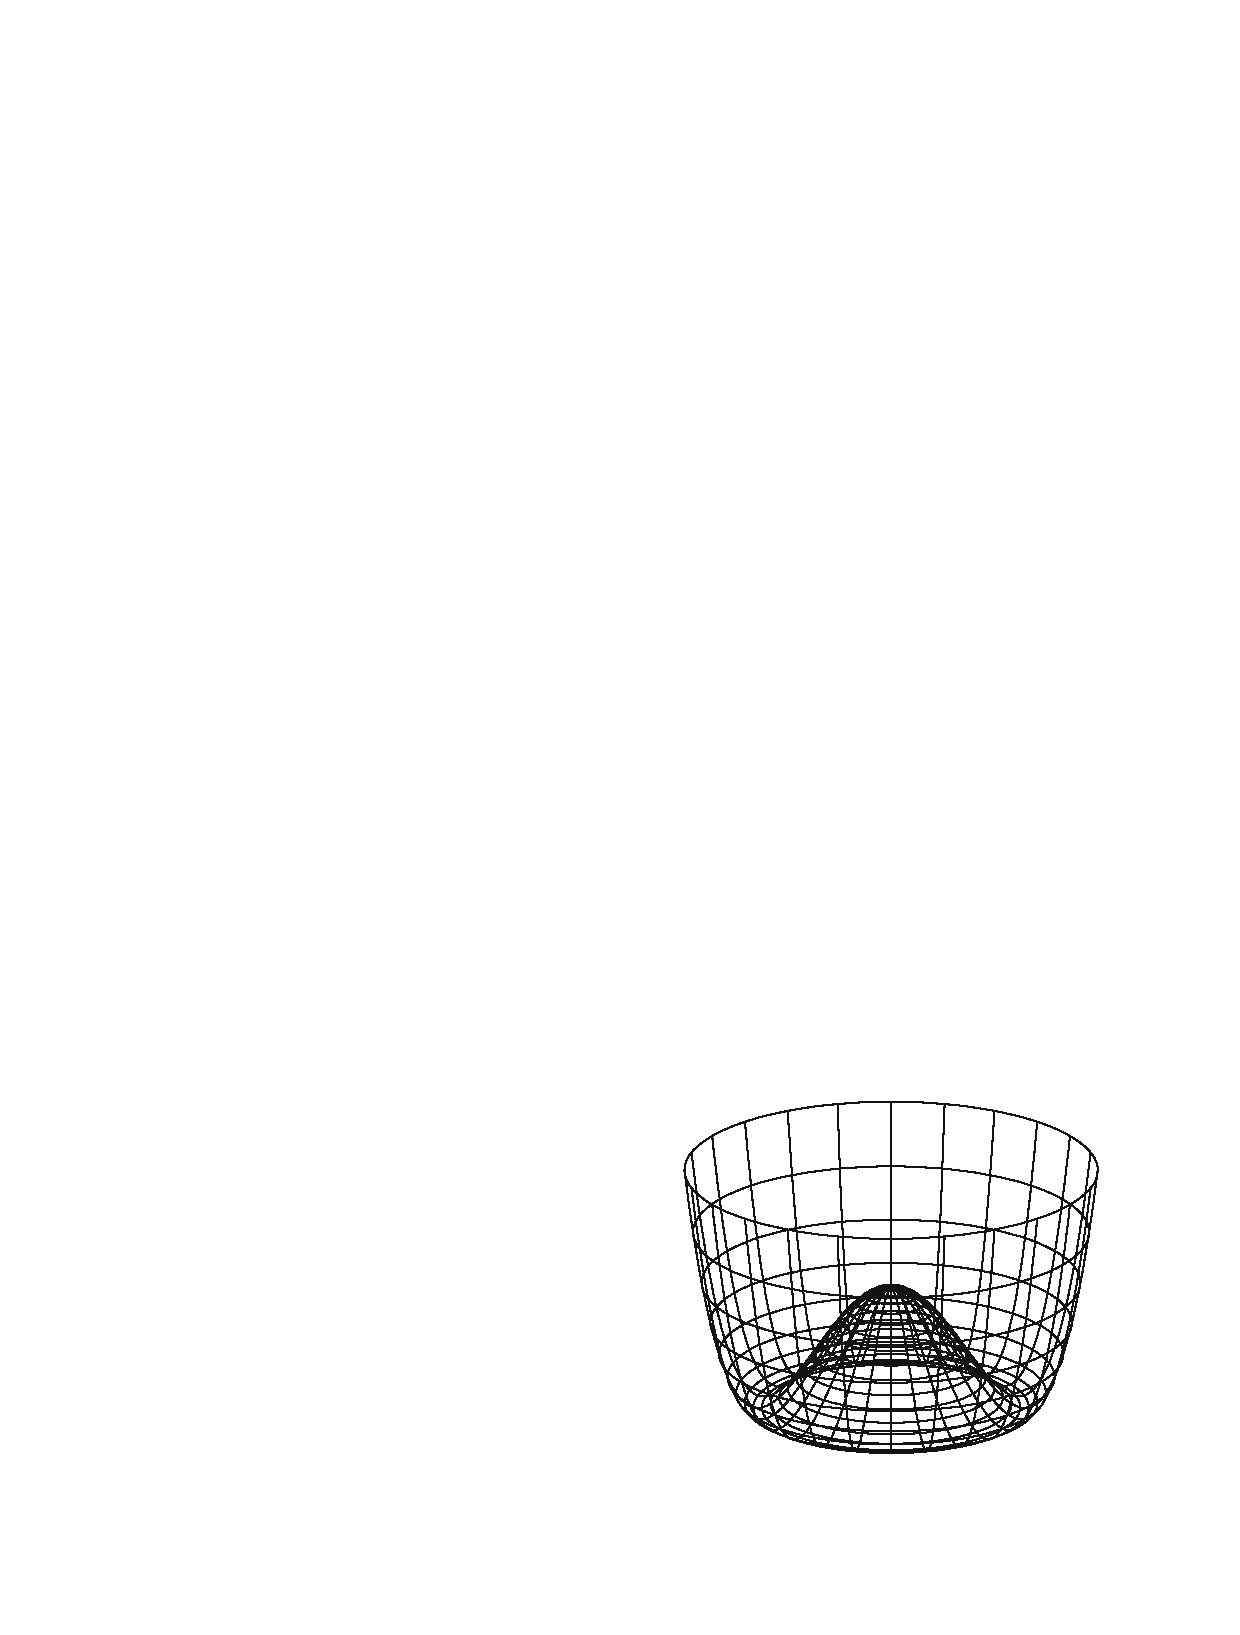
\includegraphics[width=0.5\textwidth]{Higgs_potential}
\caption[The Higgs field potential]{The Higgs field potential in the complex plane, commonly referred to as a
``Mexican hat'' potential \autocite{top_quark_at_HC}}
\label{fig:higgs_potential}
\end{figure}

The choice of minimum corresponding to the lowest energy state (or vacuum) is completely arbitrary. In fact, any point
at which the potential is minimum loses the invariance under $SU(2)_L \times U(1)_Y$ gauge transformations. Therefore,
nature spontaneously breaks the symmetry by picking the vacuum from the set of minima of the Higgs potential.
Conventionally, we can choose
\begin{equation}
\langle 0 | \phi | 0 \rangle = \frac{1}{\sqrt{2}} \twovector{0}{v}.
\label{eq:unitary_gauge_vev}
\end{equation}

Expanding around the chosen minimum, $\phi$ is then given by
\begin{equation}
\phi = \frac{1}{\sqrt{2}} \twovector{0}{v+H},
\end{equation}
where $H$ is the neutral scalar Higgs field. By substituting this field into the Lagrangian in
Equation~\ref{eq:Higgs_L}, one can obtain:
\begin{equation}
\begin{split}
\calL_\textrm{Higgs} & = \frac{1}{2} (\partial_\mu H)(\partial^\mu H) + \frac{1}{4} g^2 (H^2 + 2vH + v^2) W^+_\mu
W^{-\mu} + \\ & + \frac{1}{8} (g^2 + {g'}^2)(H^2 + 2vH + v^2)Z_\mu Z^\mu - \\ & - \mu^2 H^2 - \frac{\lambda}{4} (H^4 +
4vH^3),
\end{split}
\label{eq:Higgs_L_final}
\end{equation}
where physical fields $W^{\pm}_\mu$ and $Z_\mu$ are given by Equations~\ref{eq:W_mu} and \ref{eq:Z_mu}, respectively.
Notably, we can see that these fields have acquired mass terms in the Lagrangian, with the masses of vector bosons given
by
\begin{subequations}
\begin{align}
M_W &= \frac{1}{2}gv, \\
M_Z &= \frac{1}{2}v\sqrt{g^2+{g'}^2} = \frac{1}{2} \frac{gv}{\cos{\theta_W}},
\end{align}
\end{subequations}
whereas the mass of the Higgs boson itself is given by
\begin{equation}
M_H = \sqrt{2} \mu = v \sqrt{2\lambda}.
\end{equation}

% Unlike the \W and \Z boson masses which can be predicted from the measurement of the fine structure constant, the Higgs
% mass $M_H$ can not be determined by other experimentally measured parameters.

% However, it is possible to put indirect constraints on $M_H$ through quantum loop corrections and precise measurement of
% the \W boson and top quark masses. This will be discussed in Section~\ref{s:top_quak_physics}.

Naturally, the photon field $A_\mu$ acquires no mass terms in the Lagrangian. The Higgs mechanism can also be used in a
similar way to generate fermion masses by introducing an $SU(2)_L \times U(1)_Y$ gauge invariant term responsible for
interaction between the Higgs and fermion fields. This additional term in the Standard Model Lagrangian is called the
\textit{Yukawa term}, which for the first generation of fermions is given by
\begin{equation}
\calL_\textrm{Yukawa} = -Y_e^{ij} \bar{l_L}^i \phi e_R^j - Y_u^{ij} \bar{q_L}^i \epsilon \phi^\dag u_R^j - Y_d^{ij}
\bar{q_L}^i \phi d_R^j + \textrm{h.c.},
\end{equation}
where coefficients $Y_{e,u,d}^{ij}$ are $3\times3$ complex matrices (Yukawa couplings) and $\epsilon$ is the $2\times2$
antisymmetric tensor. When the Higgs field $\phi$ acquires the vacuum expectation value given by
Equation~\ref{eq:unitary_gauge_vev}, the Yukawa Lagrangian yields mass terms for fermions, generating the masses:
\begin{equation}
M_f = Y_f \frac{v}{\sqrt{2}}.
\end{equation}

The Yukawa couplings are not diagonal in general, which results in mixing between different generations described for
the quarks by the CKM matrix (Equation~\ref{eq:CKM}). Another curious observation is that the fermion masses are
proportional to Yukawa couplings, which essentially represent the interaction strength with the Higgs field. Due to the
large mass of the top quark of approximately \SI{173}{\GeV}, and the Higgs field vacuum expectation value
$v\approx\SI{246}{\GeV}$, the Yukawa coupling to the top quark is very close to unity.

The existence of the Higgs boson and therefore the nature of electroweak symmetry breaking had long remained a mystery.
In the summer of 2012 both ATLAS and CMS experiments at the LHC observed a Higgs boson with an approximate mass of
\SI{125}{\GeV} \autocite{ATLAS_higgs_observation, CMS_higgs_observation}, with couplings consistent with theoretical
predictions \autocite{CMS_Higgs_long_paper, ATLAS_Higgs_couplings}, which proved to be yet another triumph of the
Standard Model.

\newpage
\subsection{Shortcomings of the SM and physics beyond it}
\label{ss:SM_shortcomings}
Despite being the most successful theory to date, the Standard Model is not perfect and has its shortcomings. There is a
range of physical phenomena not explained by the SM. Let us mention the most prominent ones.

\begin{description}[wide=\parindent]
\item [Gravity] is not included in the Standard Model, as a consistent theory of quantum gravity is yet to be derived.
General relativity, the only accepted theory of gravity, is in fact incompatible with quantum mechanics and therefore
the Standard Model.
\item [Massive neutrinos] are also not explained by the SM. The evidence for neutrino oscillations was confirmed by the
Super-Kamiokande collaboration \autocite{neutrino_oscillations}, which necessarily implies that neutrinos are massive
particles. It is possible to include massive neutrinos in some extensions of the Standard Model, whilst also keeping the
local symmetry of weak interactions \autocite{Shaposhnikov_nuMSM}. However, this leads to new theoretical problems
(e.g.\ unnaturally small neutrino Yukawa couplings).
\item [Matter/antimatter asymmetry,] which is apparent in the Universe, is not fully accounted for by the observed CP
violation in the Standard Model \autocite{Peskin_matter_antimatter, matter_antimatter_asymmetry}. Therefore, another
mechanism inducing the matter/antimatter asymmetry must exist, most likely requiring new physics models beyond the
Standard Model.

%\item [Strong CP problem] refers to the absence of any fundamental theoretical prohibition of CP violation in strong
%interactions. However, such strong CP violation has not been observed.
\item [Dark matter and dark energy] constitute approximately \SI{95}{\pc} of the mass and energy content in our
Universe, according to the latest Planck data \autocite{planck2013-p01, planck2013-p11}. The Standard Model only
describes the remaining \SI{5}{\pc} (i.e.\ ordinary matter), whereas the origin of dark matter and dark energy remains
unknown.
\end{description}

Furthermore, there are a number of fundamental theoretical issues within the Standard Model, implying the intrinsic
incompleteness of the theory. The SM does not explain why it has only three generations of fermions. Moreover, there is
no explanation for the vast difference between masses of fermions (known as the Flavour problem), hence the origin of
Yukawa couplings (and therefore the CKM matrix) remains an open problem in particle physics.

Additionally, the \textit{ad hoc} nature of the Higgs mechanism gives rise to the hierarchy problem, which is related to
quadratic divergence of the loop corrections to the Higgs boson mass. The Higgs mass is renormalised by loop diagrams
(e.g.\ shown in Figure~\ref{fig:Higgs_loops}), making it extremely large  -- of the order of Planck scale (\SI{\sim
e19}{\GeV}) -- unless there is some unnatural fine tuning involved.

\begin{figure}[!hbtp]
	\centering
	\begin{minipage}[b]{0.4\textwidth}
	\centering
	\subfloat[]{
		\begin{fmfgraph*}(100,50)
		\fmfleft{i}
		\fmfright{o}
		\fmflabel{$H$}{i}
		\fmflabel{$H$}{o}
		\fmf{dashes,tension=3}{i,v1}
		\fmf{dashes,tension=3}{v2,o}
		\fmf{fermion,left,tension=1}{v1,v2,v1}
		\fmfdot{v1,v2}
		\end{fmfgraph*}
	}
	\end{minipage}
	\hspace{1cm}
	\begin{minipage}[b]{0.4\textwidth}
	\centering
	\subfloat[]{
		\begin{fmfgraph*}(100,50)
		\fmfleft{i}
		\fmfright{o}
		\fmflabel{$H$}{i}
		\fmflabel{$H$}{o}
		\fmf{dashes}{i,v1}
		\fmf{dashes}{v1,o}
		\fmffreeze
		\fmf{dashes,tension=1}{v1,v1}
		\fmfdot{v1}
		\end{fmfgraph*}
	}
	\end{minipage}
	\caption[Loop contributions to the Higgs boson mass]{Loop contributions to the Higgs boson mass: (a) fermion loops, (b)
	boson loops.}
  \label{fig:Higgs_loops}
\end{figure}


All these problems motivate the need for new models, referred to as physics beyond the Standard Model (BSM). Most
notable BSM models are briefly mentioned below.

\begin{description}[wide=\parindent]
\item [Supersymmetry] (SUSY) \autocite{SUSY_primer} is an extension of the SM, introducing a supersymmetric partner to
each ordinary particle by varying its spin by $1/2$. Thus, each fermion has a bosonic partner, and all bosons have
fermionic partners. Despite the greater number of free parameters, SUSY offers attractive solutions to most of the
mentioned problems of the SM. For example, the hierarchy problem is naturally solved in SUSY since the loop corrections
are automatically cancelled by corresponding contributions from supersymmetric partners. Most SUSY models also provide
good candidates for Dark Matter.
\item [Extra dimensions] refer to theories containing additional space-time dimensions, in which gravity is allowed to
propagate. This leads to a reduction of the hierarchy between the Planck and electroweak scales, thus resolving the
hierarchy problem \autocite{Arkani-Hamed, RS}.
\item [Composite models,] such as topcolour \autocite{topcolour} or composite Higgs \autocite{composite_Higgs} models,
attempt to resolve some of the issues of the Standard Model by either introducing new composite particles or suggesting
a composite nature for the existing particles in the SM.
%\item [Grand Unified Theories (GUTs)] are a range of models striving to unify all fundamental forces.
\end{description}

An important and desirable feature of any physics model is its falsifiability in the accessible energy range. A variety
of BSM models provide particle candidates that may exhibit themselves at the energy scale accessible at the LHC,
therefore a rich physics programme at the LHC must ensure an active search for all possible signs of new physics.

\newpage
\section{Top Quark Physics within the Standard Model}
\label{s:top_quak_physics}
The top quark is the heaviest elementary particle in the Standard Model, and the heaviest observed particle, discovered
in 1995 at the Tevatron collider by the CDF and D{\O} collaborations \autocite{CDF_top_observation, D0_top_observation}.
Its large mass of approximately \SI{173}{\GeV} suggests that the top quark may have a special role in nature. It is
substantially more massive than any other fermion. As mentioned in Section~\ref{ss:SM_shortcomings}, the reason for such
vast discrepancy between fermion masses is unknown. It is also not yet understood why the top quark's Yukawa coupling to
the Higgs boson is so close to unity. Naturally, studying the most massive fermion is a logical starting point in search
for answers to these questions.

Due to its large mass, the top quark has an extremely short lifetime on the order of \SI{e-25}{\s} \autocite{PDG},
meaning that it decays before the top-flavoured hadrons or \ttbar bound states can form. Therefore, the spin information
is passed from the top quark on to its decay products, providing a unique possibility to study a ``bare'' quark.
High-precision measurements of the top quark properties, such as mass (Chapter~\ref{c:top_mass_analysis}) and cross
section (Chapter~\ref{c:xsection_analysis}) are important tools to test the Standard Model and probe for new physics
beyond it.

\subsection{Top quark production at the LHC}
\label{ss:top_production}
There are two particular mechanisms of top quark production in hadron collisions: top-antitop (\ttbar) pair production
via the strong interaction, and single top quark production via the electroweak interaction. The \ttbar production
dominates over single top production, being the main source of top quarks at the LHC, and therefore is the main focus of
this thesis.

Feynman diagrams for leading order \ttbar production are presented in
Figure~\ref{fig:ttbar_production_feynman_diagrams}. Since the LHC is a proton-proton collider with a high centre of mass
energy, the only source of antiquarks are virtual quarks (so-called sea quarks), and the gluon contribution becomes
dominating. Therefore, the major process for \ttbar production is gluon fusion, constituting approximately \SI{90}{\pc}
(\SI{80}{\pc}) at $\sqrt s =$ \SI{14}{\TeV} (\SI{7}{\TeV}) \autocite{PDG}. Quark-antiquark annihilation and higher-order
processes contribute the rest of the Standard Model \ttbar production. At the proton-antiproton Tevatron, on the
contrary, the quark-antiquark annihilation was the main \ttbar production mode.

\begin{figure}[!htbp]
	\begin{minipage}[t]{0.49\textwidth}
	\centering
	\subfloat[]{
		\begin{fmfgraph*}(150,75)
		\fmfleft{i1,i2}
		\fmfright{o1,o2}
		\fmflabel{$g$}{i1}
		\fmflabel{$g$}{i2}
		\fmflabel{$\bar{t}$}{o1}
		\fmflabel{$t$}{o2}

		\fmf{gluon}{i1,v1}
		\fmf{gluon}{i2,v2}
		\fmf{fermion}{v1,v2}
		\fmf{fermion}{o1,v1}
		\fmf{fermion}{v2,o2}
		\end{fmfgraph*}
	}
	\end{minipage}
	\hfill
	\begin{minipage}[t]{0.49\textwidth}
	\centering
	\subfloat[]{
		\begin{fmfgraph*}(150,75)
		\fmfleft{i1,i2}
		\fmfright{o1,o2}
		\fmflabel{$g$}{i1}
		\fmflabel{$g$}{i2}
		\fmflabel{$\bar{t}$}{o1}
		\fmflabel{$t$}{o2}

		\fmf{gluon}{i1,v1}
		\fmf{gluon}{i2,v1}
		\fmf{gluon}{v1,v2}
		\fmf{fermion}{o1,v2}
		\fmf{fermion}{v2,o2}
		\end{fmfgraph*}
	}
	\end{minipage}

	\vspace{1cm}

	\begin{minipage}[t]{0.49\textwidth}
	\centering
	\subfloat[]{
		\begin{fmfgraph*}(150,75)
		\fmfleft{i1,i2}
		\fmfright{o1,o2}
		\fmflabel{$g$}{i1}
		\fmflabel{$g$}{i2}
		\fmflabel{$\bar{t}$}{o1}
		\fmflabel{$t$}{o2}

		\fmf{gluon}{i1,v1}
		\fmf{phantom}{v1,o1}
		\fmf{gluon}{i2,v2}
		\fmf{phantom}{v2,o2}
		\fmf{fermion}{v2,v1}

		\fmf{fermion,tension=0}{v1,o2}
		\fmf{fermion,tension=0}{o1,v2}

		\end{fmfgraph*}
	}
	\end{minipage}
	\hfill
	\begin{minipage}[t]{0.49\textwidth}
	\centering
	\subfloat[]{
		\begin{fmfgraph*}(150,75)
		\fmfleft{i1,i2}
		\fmfright{o1,o2}
		\fmflabel{$\bar{q}$}{i1}
		\fmflabel{$q$}{i2}
		\fmflabel{$\bar{t}$}{o1}
		\fmflabel{$t$}{o2}

		\fmf{fermion}{v1,i1}
		\fmf{fermion}{i2,v1}
		\fmf{gluon}{v1,v2}
		\fmf{fermion}{o1,v2}
		\fmf{fermion}{v2,o2}
		\end{fmfgraph*}
	}
	\end{minipage}

	\caption[Feynman diagrams for leading order \ttbar production at the LHC]{Feynman diagrams for leading order \ttbar
	production at the LHC: (a), (b) and (c) show the gluon fusion, the dominant production mechanism, (d) represents
	quark-antiquark annihilation.}
  \label{fig:ttbar_production_feynman_diagrams}
\end{figure}

Figure~\ref{fig:single_top_production_feynman_diagrams} shows the Feynman diagrams of single top production modes. Three
major production mechanisms include \cPqs-channel and \cPqt-channel \W boson exchange, and associated production with a
\W boson (\tW-channel). Measurement of single top production is of significant interest since it allows the direct
measurement of the Wtb vertex and therefore the magnitude of the $|\Vtb|$ element of the CKM matrix.

\begin{figure}[!hbtp]
	\centering
	\vspace*{0.5cm}
	\begin{minipage}[b]{0.3\textwidth}
	\centering
	\subfloat[]{
		\begin{fmfgraph*}(150,75)
		\fmfleft{i1,i2}
		\fmfright{o1,o2}
		\fmflabel{$q$}{i1}
		\fmflabel{$\bar{q}'$}{i2}
		\fmflabel{$\bar{b}$}{o1}
		\fmflabel{$t$}{o2}

		\fmf{fermion}{i1,v1}
		\fmf{fermion}{v1,i2}
		\fmf{photon, label=$W$}{v1,v2}
		\fmf{fermion}{o1,v2}
		\fmf{fermion}{v2,o2}
		\end{fmfgraph*}
	}
	\end{minipage}
	\hfill
	\begin{minipage}[b]{0.3\textwidth}
	\centering
	\subfloat[]{
		\begin{fmfgraph*}(150,75)
		\fmfleft{i1,i2}
		\fmfright{o1,o2,o3}
		\fmflabel{$g$}{i1}
		\fmflabel{$q$}{i2}
		\fmflabel{$\bar{b}$}{o1}
		\fmflabel{$t$}{o2}
		\fmflabel{$q'$}{o3}

		\fmf{gluon}{i1,v1}
		\fmf{fermion}{i2,v3}
		\fmf{fermion, label=$b$}{v1,v2}
		\fmf{photon, label=$W$}{v2,v3}
		\fmf{fermion}{o1,v1}
		\fmf{fermion}{v2,o2}
		\fmf{fermion}{v3,o3}
		\end{fmfgraph*}
	}
	\end{minipage}
	\hfill
	\begin{minipage}[b]{0.3\textwidth}
	\centering
	\subfloat[]{
		\begin{fmfgraph*}(150,75)
		\fmfleft{i1,i2}
		\fmfright{o1,o2}
		\fmflabel{$b$}{i1}
		\fmflabel{$q$}{i2}
		\fmflabel{$t$}{o1}
		\fmflabel{$q'$}{o2}

		\fmf{fermion}{i1,v1}
		\fmf{fermion}{i2,v2}
		\fmf{photon, label=$W$}{v1,v2}
		\fmf{fermion}{v1,o1}
		\fmf{fermion}{v2,o2}
		\end{fmfgraph*}
	}
	\end{minipage}

	\vspace{1cm}

	\hfill

	\begin{minipage}[t]{0.3\textwidth}
	\centering
	\subfloat[]{
		\begin{fmfgraph*}(150,75)
		\fmfleft{i1,i2}
		\fmfright{o1,o2}
		\fmflabel{$g$}{i1}
		\fmflabel{$b$}{i2}
		\fmflabel{$t$}{o1}
		\fmflabel{$W$}{o2}

		\fmf{gluon}{i1,v1}
		\fmf{fermion}{i2,v1}
		\fmf{fermion, label=$b$}{v1,v2}
		\fmf{fermion}{v2,o1}
		\fmf{photon}{v2,o2}
		\end{fmfgraph*}
	}
	\end{minipage}
	\hspace{2cm}
	\begin{minipage}[t]{0.3\textwidth}
	\centering
	\subfloat[]{
		\begin{fmfgraph*}(150,75)
		\fmfleft{i1,i2}
		\fmfright{o1,o2}
		\fmflabel{$b$}{i1}
		\fmflabel{$g$}{i2}
		\fmflabel{$W$}{o1}
		\fmflabel{$t$}{o2}

		\fmf{fermion}{i1,v1}
		\fmf{gluon}{i2,v2}
		\fmf{fermion, label=$t$}{v1,v2}
		\fmf{photon}{v1,o1}
		\fmf{fermion}{v2,o2}
		\end{fmfgraph*}
	}
	\end{minipage}
	\hfill

	\caption[Feynman diagrams for leading order single top production]{Feynman diagrams for leading order
	single top production. (a) s-channel, (b) and (c) t-channel, (d) and (e) tW-channel.}
  \label{fig:single_top_production_feynman_diagrams}
\end{figure}

\subsection{Top quark decay}
\label{ss:top_decay}
The top quark predominantly decays to a \W boson and a b-quark: $\cPqt \rightarrow \W \cPqb$. Other possible decay modes
($\cPqt \rightarrow \W \cPqs$ and $\cPqt \rightarrow \W \cPqd$) are suppressed in the Standard Model by the unitarity
requirement of the CKM matrix, which yields \autocite{PDG} the $|\Vtb|$ value of
\begin{equation}
|\Vtb| = 0.999146^{+0.000021}_{-0.000046}.
\end{equation}

As already mentioned, the direct measurement of $|\Vtb|$ (without assuming unitarity) can be performed by measuring
the single top production cross section. The recent CMS result is consistent with the Standard Model
\autocite{single_top_Vtb_CMS}:
\begin{equation}
|\Vtb| = 0.998 \pm 0.038~\textrm{(experimental)} \pm 0.016~\textrm{(theoretical)}.
\end{equation}

The branching fraction of $\cPqt \rightarrow \W \cPqb$ decay is assumed to be \SI{100}{\pc} hereafter. Therefore, the
\ttbar decay modes completely depend on subsequent \W boson decays:
\begin{itemize}
  \item fully hadronic: \ttbar $\rightarrow \cPqb \W^+ ~ \bar{\cPqb} \W^- \rightarrow  \cPqb~\cPq\bar{\cPq}' ~
  \bar{\cPqb}~\cPq'' \bar{\cPq}'''$ (\SI{45.7}{\pc});
  \item semileptonic: \ttbar $\rightarrow \cPqb \W^+ ~ \bar{\cPqb} \W^- \rightarrow \cPqb~\cPq\bar{\cPq}' ~ \bar{\cPqb}
  ~ l^- \bar{\nu}_l + \cPqb~l^+ \nu_l ~ \bar{\cPqb}~\cPq'' \bar{\cPq}'''$ (\SI{43.8}{\pc});
  \item dileptonic: \ttbar $\rightarrow \cPqb \W^+ ~ \bar{\cPqb} \W^- \rightarrow  \cPqb~\bar{l} \nu_l ~ \bar{\cPqb} ~
  l'\bar{\nu}_{l'}$ (\SI{10.5}{\pc}).
\end{itemize}

Percentages in parentheses show the branching fractions corresponding to the decay modes \autocite{PDG}. The quarks in
all final states hadronise into jets. The number of jets is not limited to the number of initial quarks due to the
contribution from extra QCD radiation (i.e.\ gluon radiation) either before or after \ttbar production.

The fully hadronic \ttbar decay signature implies at least six jets in the final state and no leptons, hence it is
heavily contaminated by the background from QCD and \W/\ZpJets processes. Dileptonic \ttbar decay has a clean signature,
but due to the lowest branching fraction can suffer from limited statistics. The semileptonic decay mode, shown in
Figure~\ref{fig:ttbar_semileptonic_decay}, has exactly one highly energetic lepton and at least four jets in the final
state, which is therefore called the lepton plus jets final state. The lepton can be an electron, a muon or a
$\tau$-lepton; however, since the $\tau$-leptons are difficult to reconstruct, they are usually excluded from top quark
analyses studying semileptonic decays. Analyses in this thesis study the electron plus jets ($e+$jets) and muon plus
jets ($\mu+$jets) decay channels, which have branching fractions of about \SI{14}{\pc} each.

\begin{figure}[!hbtp]
	\centering
	\vspace*{0.5cm}
	\begin{fmfgraph*}(300,150)
	\fmfleft{i1,i2,i3}
	\fmfright{o1,o2,o3}
	\fmflabel{$\bar{q}$}{i1}
	\fmflabel{$q$}{i2}
	\fmflabel{$\bar{b}$}{i3}
	\fmflabel{$b$}{o1}
	\fmflabel{$l^+$}{o2}
	\fmflabel{$\nu_l$}{o3}
	
	\fmf{fermion}{i3,v2}
	\fmf{phantom}{i1,v2}
	\fmf{fermion, label=$\bar{t}$}{v2,v3}
	\fmf{fermion, label=$t$}{v3,v4}
	\fmf{fermion}{v4,o1}
	\fmf{phantom}{o3,v4}
	\fmffreeze
	\fmf{fermion}{i1,v1}
	\fmf{fermion}{v1,i2}
	\fmf{fermion}{o2,v5}
	\fmf{fermion}{v5,o3}
	\fmf{photon, label=$W^-$}{v1,v2}
	\fmf{photon, label=$W^+$}{v4,v5}
	\fmfdot{v3}
	\end{fmfgraph*}
	\caption{Semileptonic \ttbar decay mode}
  \label{fig:ttbar_semileptonic_decay}
\end{figure}


\newpage
\subsection{Background processes to semileptonic top quark pair decay}
\label{ss:backgrounds}
Both top quark mass and differential cross section analyses presented in this thesis are based on a selection of events
with semileptonic ($e/\mu+$jets) \ttbar decay signature. Being relatively clean yet still providing sufficient event
yields, this decay mode is used in many measurements of top quark properties. Good understanding of background
contributions is very important for accuracy and reliability of measurements. The most significant background processes
to semileptonic \ttbar decay are described below.

\subsubsection*{Single top quark background}
One of the less significant backgrounds to lepton plus jets analyses is the single top quark production. Major
production modes for this process (mentioned in Section~\ref{ss:top_production}) have a lower number of jets in the
final state than that of the \ttbar production, however, additional jets can emerge from initial and final state
radiation (ISR/FSR), i.e.\ soft gluon radiation before and after the hard scattering process. This contribution is not
negligible, and is modelled using Monte Carlo simulation.

\subsubsection*{\WpJets background}
Production of \W bosons with additional jets (called \WpJets) is one of the most significant backgrounds to semileptonic
\ttbar decays. Example Feynman diagrams for leading order \W boson production are shown in
Figure~\ref{fig:VJets_processes} (a, b). Leptonic decays in the \WpJets process together with extra jets can
successfully mimic the \ttbar decay since it also includes two \W bosons. However, leptons and jets in \WpJets processes
are usually much softer than those coming from \ttbar decay, due to the large mass of top quarks. Moreover, additional
jets are less likely to be \cPqb-jets which are necessarily present in \ttbar decay. Therefore, tagging of \cPqb-jets
and high kinematic cuts on lepton and jets transverse momenta can significantly reduce the
\WpJets background. Besides, the production cross section of \WpJets events reduces exponentially with increasing number
of jets \autocite{multijet_WZ}, therefore jet multiplicity cuts also help to mitigate this background. These methods are
detailed in the selection procedures of top quark mass and differential cross section analyses in
Sections~\ref{s_top_mass:event_selection} and \ref{s_xsection:event_selection}, respectively.

\subsubsection*{\ZpJets background}
\Z boson production processes with additional jets (\ZpJets) are largely similar to \WpJets processes, as can be seen in
Figure~\ref{fig:VJets_processes} (c, d). The difference lies in leptonic decays of the \Z boson, as it produces two
opposite-sign leptons. Vetoing the second lepton in the selection is therefore particularly helpful in reducing this
background. Contamination can still occur if one of the leptons is misreconstructed as a jet or does not pass
identification criteria. This contribution is estimated to be small, and together with the jet multiplicity cuts the
\ZpJets background is usually mitigated significantly.

\begin{figure}[tbp]
	\begin{minipage}[t]{0.49\textwidth}
	\centering
	\subfloat[]{
		\begin{fmfgraph*}(150,75)
		\fmfleft{i1,i2}
		\fmfright{o1,o2}
		\fmflabel{$q$}{i1}
		\fmflabel{$g$}{i2}
		\fmflabel{$q'$}{o1}
		\fmflabel{$W$}{o2}

		\fmf{fermion}{i1,v1}
		\fmf{gluon}{i2,v1}
		\fmf{fermion}{v1,v2}
		\fmf{fermion}{v2,o1}
		\fmf{photon}{v2,o2}
		\end{fmfgraph*}
	}
	\end{minipage}
	\hfill
	\begin{minipage}[t]{0.49\textwidth}
	\centering
	\subfloat[]{
		\begin{fmfgraph*}(150,75)
		\fmfleft{i1,i2}
		\fmfright{o1,o2}
		\fmflabel{$q$}{i1}
		\fmflabel{$\bar{q}'$}{i2}
		\fmflabel{$g$}{o1}
		\fmflabel{$W$}{o2}

		\fmf{fermion}{i1,v1}
		\fmf{fermion}{v2,i2}
		\fmf{fermion}{v1,v2}
		\fmf{gluon}{v1,o1}
		\fmf{photon}{v2,o2}
		\end{fmfgraph*}
	}
	\end{minipage}

	\vspace{1cm}

	\begin{minipage}[t]{0.49\textwidth}
	\centering
		\subfloat[]{
		\begin{fmfgraph*}(150,75)
		\fmfleft{i1,i2}
		\fmfright{o1,o2}
		\fmflabel{$q$}{i1}
		\fmflabel{$g$}{i2}
		\fmflabel{$q'$}{o1}
		\fmflabel{$Z$}{o2}

		\fmf{fermion}{i1,v1}
		\fmf{gluon}{i2,v1}
		\fmf{fermion}{v1,v2}
		\fmf{fermion}{v2,o1}
		\fmf{photon}{v2,o2}
		\end{fmfgraph*}
	}
	\end{minipage}
	\hfill
	\begin{minipage}[t]{0.49\textwidth}
	\centering
	\subfloat[]{
		\begin{fmfgraph*}(150,75)
		\fmfleft{i1,i2}
		\fmfright{o1,o2}
		\fmflabel{$g$}{i1}
		\fmflabel{$q$}{i2}
		\fmflabel{$q'$}{o1}
		\fmflabel{$Z$}{o2}

		\fmf{gluon}{i1,v1}
		\fmf{fermion}{i2,v2}
		\fmf{fermion}{v2,v1}
		\fmf{fermion}{v1,o1}
		\fmf{photon}{v2,o2}
		\end{fmfgraph*}
	}
	\end{minipage}

	\caption[Example diagrams for leading order \W and \Z boson production at the
	LHC.]{Example diagrams for leading order \W boson (a, b) and \Z boson (c,
	d) production at the LHC.}
  \label{fig:VJets_processes}
\end{figure}

\subsubsection*{QCD multi-jet background}
Standard QCD processes in hadron collisions, such as gluon fusion and quark-antiquark annihilation, usually result in
the production of highly energetic jets. Examples of these processes in the lowest order with two jets in the final
state are shown in Figure~\ref{fig:QCD_processes}. Additional jets arise at higher orders and can potentially fake
\ttbar signal. Although QCD events do not produce real prompt leptons, this can happen when jets are mis-identified as
leptons. These objects are referred to as fake leptons. Due to strict identification criteria of real electrons and
muons (described in Sections~\ref{ss:electron_reconstruction} and \ref{ss:muon_reconstruction}), such
mis-identifications are extremely rare. However, since the production cross section of QCD events is very large, this
background becomes non-negligible.

\begin{figure}[tbp]
	\begin{minipage}[t]{0.49\textwidth}
	\centering
	\subfloat[]{
		\begin{fmfgraph*}(150,75)
		\fmfleft{i1,i2}
		\fmfright{o1,o2}
		\fmflabel{$q$}{i1}
		\fmflabel{$g$}{i2}
		\fmflabel{$\bar{q}$}{o1}
		\fmflabel{$q$}{o2}

		\fmf{gluon}{i1,v1}
		\fmf{gluon}{i2,v1}
		\fmf{gluon}{v1,v2}
		\fmf{fermion}{o1,v2}
		\fmf{fermion}{v2,o2}
		\end{fmfgraph*}
	}
	\end{minipage}
	\hfill
	\begin{minipage}[t]{0.49\textwidth}
	\centering
	\subfloat[]{
		\begin{fmfgraph*}(150,75)
		\fmfleft{i1,i2}
		\fmfright{o1,o2}
		\fmflabel{$q$}{i1}
		\fmflabel{$g$}{i2}
		\fmflabel{$g$}{o1}
		\fmflabel{$g$}{o2}

		\fmf{gluon}{i1,v1}
		\fmf{gluon}{i2,v1}
		\fmf{gluon}{v1,v2}
		\fmf{gluon}{o1,v2}
		\fmf{gluon}{v2,o2}
		\end{fmfgraph*}
	}
	\end{minipage}

	\vspace{1cm}

	\begin{minipage}[t]{0.49\textwidth}
	\centering
		\subfloat[]{
		\begin{fmfgraph*}(150,75)
		\fmfleft{i1,i2}
		\fmfright{o1,o2}
		\fmflabel{$q$}{i1}
		\fmflabel{$g$}{i2}
		\fmflabel{$g$}{o1}
		\fmflabel{$q$}{o2}

		\fmf{fermion}{i1,v1}
		\fmf{gluon}{i2,v1}
		\fmf{fermion}{v1,v2}
		\fmf{gluon}{v2,o1}
		\fmf{fermion}{v2,o2}
		\end{fmfgraph*}
	}
	\end{minipage}
	\hfill
	\begin{minipage}[t]{0.49\textwidth}
	\centering
	\subfloat[]{
		\begin{fmfgraph*}(150,75)
		\fmfleft{i1,i2}
		\fmfright{o1,o2}
		\fmflabel{$q'$}{i1}
		\fmflabel{$q$}{i2}
		\fmflabel{$q'$}{o1}
		\fmflabel{$q$}{o2}

		\fmf{fermion}{i1,v1}
		\fmf{fermion}{i2,v2}
		\fmf{gluon}{v2,v1}
		\fmf{fermion}{v1,o1}
		\fmf{fermion}{v2,o2}
		\end{fmfgraph*}
	}
	\end{minipage}

	\caption[Example diagrams for leading order QCD multi-jet production at
	the LHC.]{Example diagrams for leading order QCD multi-jet production at
	the LHC.}
  \label{fig:QCD_processes}
\end{figure}

QCD multi-jet background is usually less significant in the muon plus jets channel, since jets faking muons are easier
to recognise. For instance, when a highly energetic jet punches through the calorimetry system into the muon chambers
and thus becomes a fake muon, it can be removed by isolation criteria as it also leaves a significant energy deposit in
the calorimeters. Muons (and electrons) can also arise from heavy flavour decays of \cPqb and \cPqc quarks -- these are
in fact real leptons, but as they don't originate at the interaction point, they can be removed by track quality cuts
most of the time.

In the electron plus jets channel, the QCD multi-jet background is more prominent. This is mainly due to photon
conversions, which occur when photons convert into electron-positron pairs. Photons can arise from prompt production
($\gamma+$jets), particle decays or bremsstrahlung radiation. Different methods for identifying such conversions have
been developed, which are discussed in detail in Section~\ref{sss:photon_conversions}.

Due to the large contribution from higher-order processes in the signal region, the QCD background is very hard to
model. Large uncertainties in theoretical cross section and potential mismodelling of higher-order effects may lead to
biases in kinematic distributions based on Monte Carlo simulation, as well as in overall acceptance of QCD events
passing the signal selection. Therefore, data-driven methods of QCD background estimation are often preferable (see
Section~\ref{s_xsection:data_driven_QCD}).

\subsubsection*{Additional backgrounds}
Other background processes potentially mimicking semileptonic \ttbar decay include the Drell-Yan process with dilepton
production ($q \bar{q} \rightarrow \Z/\gamma^* \rightarrow l \bar{l}$), and diboson production. The background
contamination from these processes can be reduced by vetoing the second lepton, and is generally considered negligible
due to the relatively small production cross sections of these processes.


\subsection{Top quark mass}
\label{ss:top_mass}
The top quark mass is a fundamental parameter of the Standard Model. However, its precise definition is a very
non-trivial problem, ultimately subject to convention. One of the most popular definitions is the pole mass,
corresponding to the real part of a pole in the perturbative propagator of a particle
\autocite{pole_mass_in_QCD_Tarrach}. For the top quark, the perturbative propagator with a four-momentum $p$ has a pole
at \autocite{top_pole_mass}:
\begin{equation}
\sqrt{p^2} = \mtop - \frac{i}{2} \Gamma_\textrm{t},
\end{equation}
where \mtop is the pole mass and $\Gamma_\textrm{t}~\SI{\approx1.5}{\GeV}$ is the top quark decay width. This definition
yields a peak in the invariant mass distribution of the top quark decay products (i.e.\ \W boson and \cPqb-quark), which
is accessible experimentally. As $\mtop \gg \Gamma_\textrm{t}/2$, the peak approximately corresponds to the pole mass,
therefore it is usually assumed that experimentally measured top quark mass represents the pole mass. As will be
discussed later, there are a few problems with this approach.

It has been shown \autocite{pole_mass_in_QCD_Kronfeld} that the pole mass is infrared finite\footnote{Infrared
finiteness corresponds to the absence of divergences due to contributions of terms with energy apporaching zero.} and
gauge-invariant to all orders of perturbative QCD. Despite being well-defined in perturbation theory, an all-order
resummation of a particular class of diagrams known as ``infrared renormalons'' \autocite{renormalons1, renormalons2}
leads to an intrinsic ambiguity of the top quark pole mass proportional to the energy scale of the strong interaction
$\Lambda_\textrm{QCD}~\SI{\approx200}{\MeV}$
\autocite{pole_MS_top_difference}.

Another frequently used mass definition which is free from renormalon ambiguity is the renormalised mass $\MSmtop(\mu)$
in the minimal subtraction (\MS) renormalisation scheme. This mass definition is often called a running mass, since it
depends on the renormalisation scale $\mu$ which is in principle arbitrary. For a choice of $\mu=\MSmtop$, the \MS mass
\MSmtop is related to the pole mass \mtop as follows \autocite{top_pole_mass}:
\begin{equation}
\mtop = \MSmtop(\MSmtop) \left( 1 + \frac{4}{3} \frac{\overline{\alpha}_S(\MSmtop)}{\pi} + 8.28
\left(\frac{\overline{\alpha}_S(\MSmtop)}{\pi} \right)^2 + ... \right) + \bigO(\Lambda_\textrm{QCD}).
\end{equation}
% \footnote{Renormalisation is a technique of cancelling divergences (infinities) in perturbative quantum field theories.
% Initially infinite parameters become finite after renormalisation, thus acquiring physical sense.}

The difference between the pole mass and the \MS mass is then estimated to be on the order of \SI{10}{\GeV} (with $\mtop
> \MSmtop$). However, it has recently been shown \autocite{pole_MS_top_difference} that including electroweak
corrections for a Higgs boson mass of \SI{\sim125}{\GeV} mostly cancels the corresponding QCD corrections, reducing the
$\mtop-\MSmtop$ difference down to \SI{\sim1}{\GeV}. Theoretical research such as studying higher-order corrections is
actively ongoing in this field.

It has been argued that the top quark mass measured at hadron colliders is in fact a parameter of Monte Carlo
generators, which does not necessarily correspond to the pole mass. This parameter is determined by (next to) leading
order calculations of the matrix elements of hard processes (see Section~\ref{s:MC_simulation}), and this mass
definition does not absorb any corrections from parton showers and hadronisation. Therefore, the actual mass definition
measured experimentally remains not fully understood, with a conceptual uncertainty on the order of
\SI{1}{\GeV} \autocite{measured_top_mass_interpretation}.

Nevertheless, experimental measurements of the top quark mass are of paramount importance. Continuously increasing
precision of the measurements is challenging the current definition of the measured mass, undoubtedly triggering more
effort in reaching a more precise theoretical specification of the mass parameter used in Monte Carlo simulation. As the
top quark is a major background to many new physics searches beyond the Standard Model, deep understanding of its mass
parameter in simulation as well as pushing down the corresponding theoretical and experimental uncertainties are
extremely important.

Another strong motivation for precise top quark mass measurement is its importance in the determination of the
electroweak vacuum stability. Measurements of both the Higgs boson and top quark masses allow extrapolating the Standard
Model Higgs potential (Equation~\ref{fig:higgs_potential}) up to Planck-scale energies. By performing a NNLO
renormalisation procedure and using the latest experimental values of \mtop and $M_H$, it has been shown
\autocite{vacuum_stability, vacuum_stability_top} that there is a significant preference for meta-stability of the SM
electroweak vacuum, as illustrated in Figure~\ref{fig:vacuum_stability}. The meta-stability corresponds to the regime
where the true minimum of the scalar potential is lower than the standard electroweak minimum, which has a lifetime
exceeding the age of the Universe. Currently the dominant uncertainty in evaluating the vacuum stability is experimental
and mostly comes from the top quark mass measurement, which provides further motivation for improved \mtop measurements.

\begin{figure}[hbtp]
   \centering
   {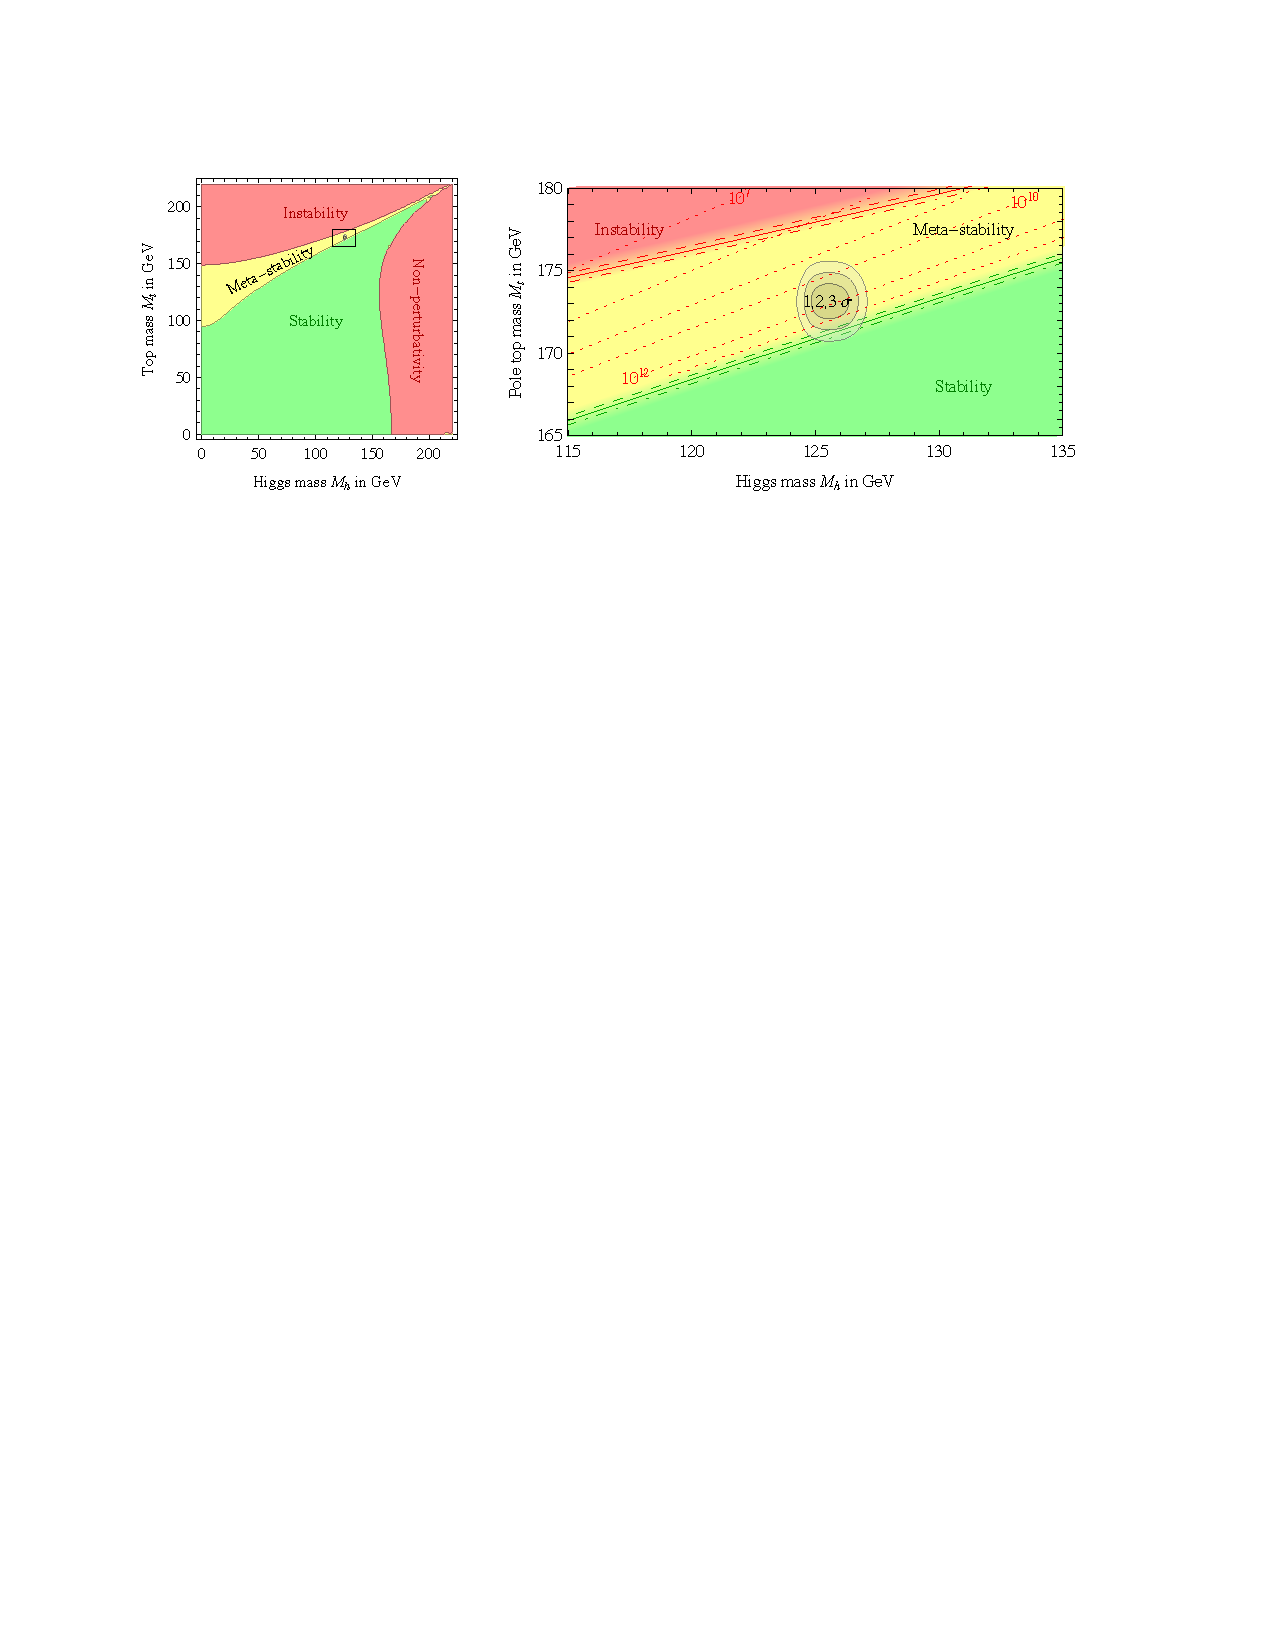
\includegraphics[width=\textwidth]{vacuum_stability}}
   \caption[The Standard Model vacuum stability]{Regions of absolute stability, meta-stability and instability of the SM
   vacuum in the \mtop/$M_H$ plane (left) and zoom into the region of the preferred experimental mass ranges. Gray areas
   show the allowed region at 1, 2 and 3 $\sigma$ \autocite{vacuum_stability}.}
   \label{fig:vacuum_stability}
\end{figure}

Nearly 20 years of the Tevatron operation resulted in a very good understanding of the machine and detectors, leading to
an impressively small systematic uncertainty on the top quark mass measurement. The latest combination result from the
Tevatron gives \autocite{tevatron_top_mass_combination}:
\begin{equation}
\mtop = 173.20 \pm 0.51~\textrm{(stat.)} \pm 0.71~\textrm{(syst.)}~\textrm{GeV}.
\end{equation}

The LHC experiments have reached nearly as good precision, with a statistical uncertainty being expectedly smaller than
that of the Tevatron, however, with a larger systematic uncertainty due to still improving understanding of detector
effects. The latest LHC combination result yields \autocite{LHC_top_mass_combination}:
\begin{equation}
\mtop = 173.29 \pm 0.23~\textrm{(stat.)} \pm 0.92~\textrm{(syst.)}~\textrm{GeV}.
\end{equation}

Recently, the first world combination result of both LHC and Tevatron measurements has become available
\autocite{world_top_mass_combination}:
\begin{equation}
\mtop = 173.34 \pm 0.27~\textrm{(stat.)} \pm 0.71~\textrm{(syst.)}~\textrm{GeV},
\end{equation}
which corresponds to a total uncertainty on the top quark mass of \SI{0.76}{\GeV}, or \SI{0.44}{\pc}. All these results
compared with contributions of individual mass measurements are shown in Figure~\ref{fig:top_mass_world_combination}.

At a proposed linear electron-positron collider (International Linear Collider, ILC), the uncertainty on the top quark
mass is expected to fall below \SI{200}{\MeV} \autocite{ILC_TDR}, i.e.\ the energy scale of the strong interaction
$\Lambda_\textrm{QCD}$. It will clearly challenge the theoretical understanding of different mass schemes, ultimately
leading to more vigorous tests of the SM and potentially providing sensitivity to new physics models.

\begin{figure}[hbtp]
   \centering
   {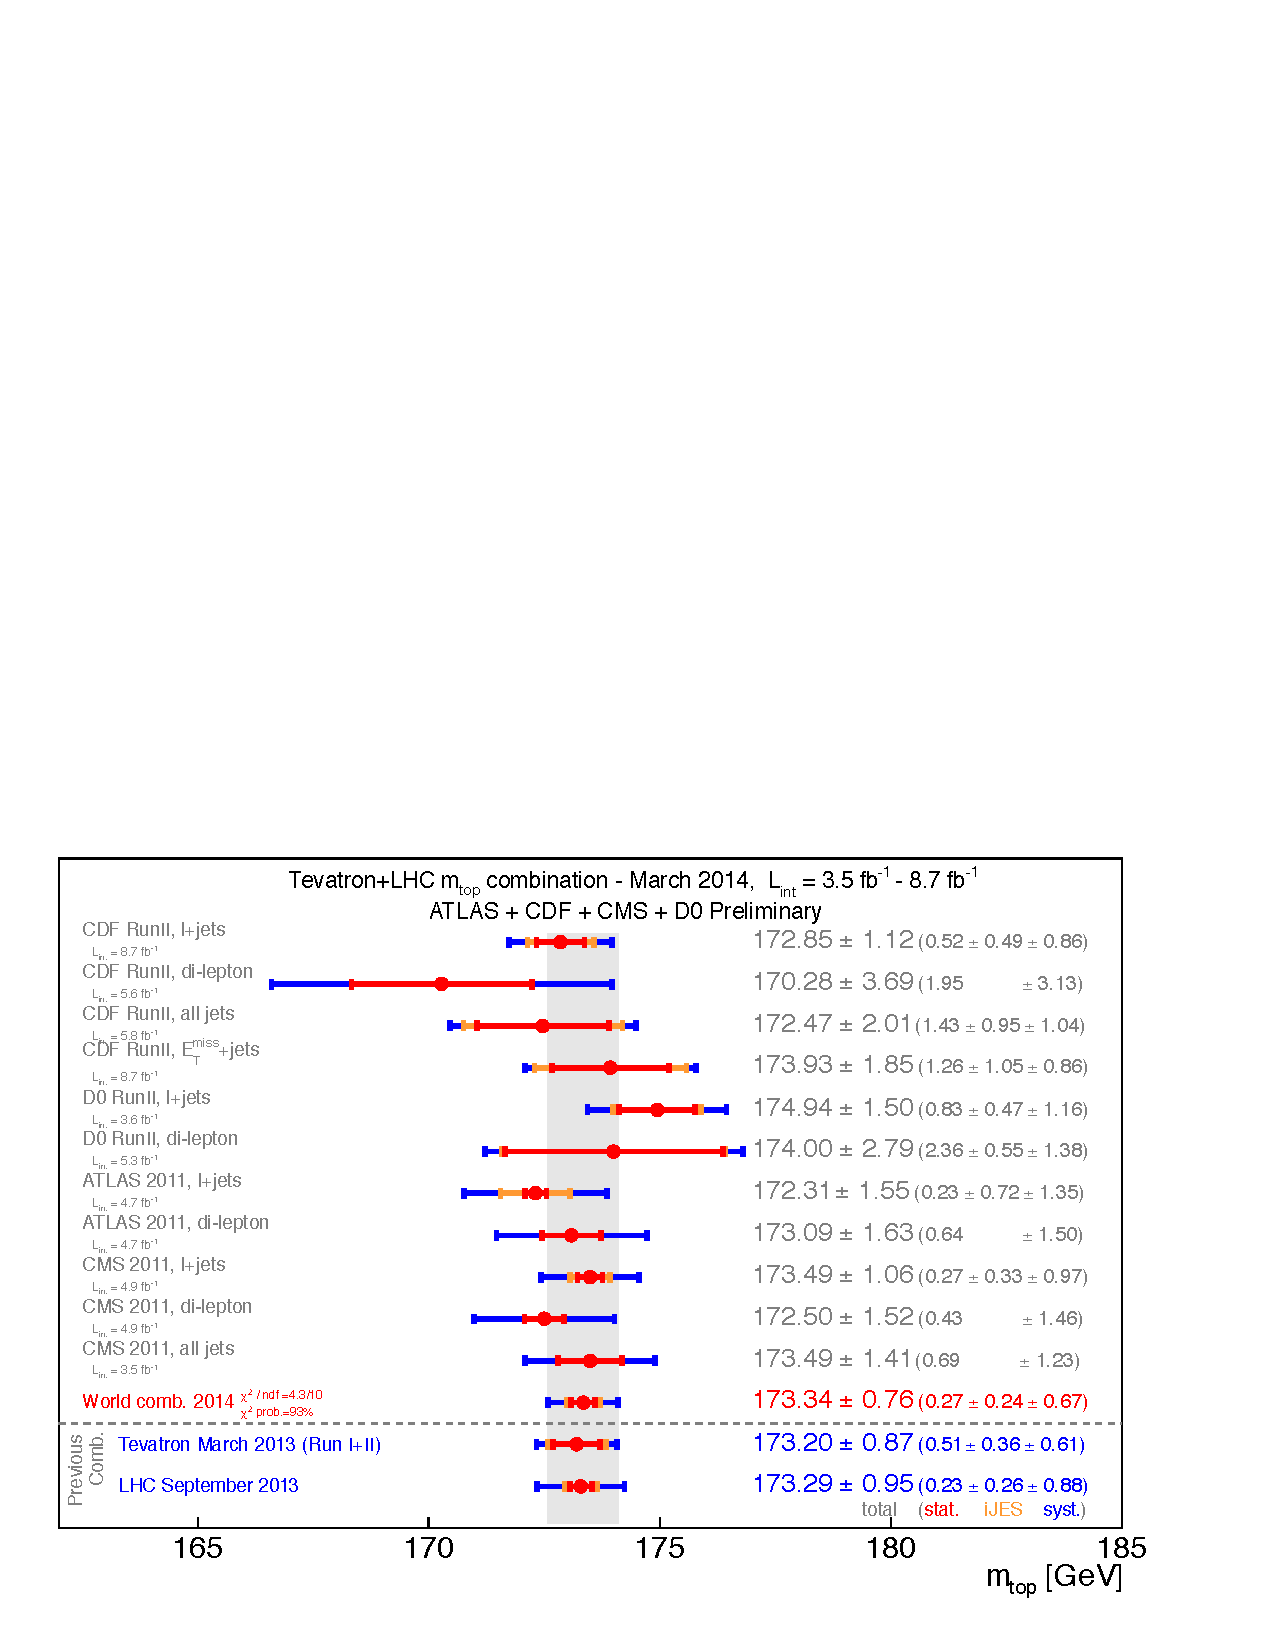
\includegraphics[width=0.9\textwidth]{top_world_combination}}
   \caption[World combination of the top quark mass measurements]{Top quark mass measurements and the result of their
   combination, compared with the Tevatron and LHC combinations. Each measurement is shown with the total uncertainty,
   the statistical, the jet energy scale (iJES, when applicable), and the systematic uncertainty. The iJES contribution
   is statistical in nature and applies only to analyses performing \textit{in situ} jet energy calibration procedures.
   The grey vertical band shows the total uncertainty on the combined value of the top quark mass
   \autocite{world_top_mass_combination}.}
   \label{fig:top_mass_world_combination}
\end{figure}

\subsection{Top quark pair production cross section}
\label{ss:ttbar_cross_section}
The \ttbar production is a strong interaction process, and therefore is described by perturbative QCD. Hadron collisions
at the LHC (or other hadron colliders) are best viewed as interactions between their constituent quarks and gluons, also
referred to as partons. Since collisions occur at high energies, these interactions result in hard scattering processes
between incoming partons, meaning those involving a significant momentum transfer comparing to the proton mass, and
potentially giving rise to highly energetic final states like top quarks. Each incoming parton carries only a fraction
$x$ of the total momentum of a parent hadron. The distribution of momentum fractions for all flavours of partons are
described by parton distribution functions (PDFs).

A PDF $f_i(x_i,\mu_f^2)$ is defined as a probability density of finding a parton with flavour $i$ and a longitudinal
momentum fraction $x_i$ when probed at momentum scale $\mu_f^2$, which is known as factorisation scale. This parameter
separates the hard scattering process into the hard partonic interaction and the soft (or long-range) interaction. The
former interaction happens at a short distance, and therefore only involves high-momentum transfer which is calculable
in perturbative QCD. The soft long-range part of the interaction, on the contrary, can not be calculated in QCD and
instead is parametrised by the PDFs, which have to be obtained from experimental data. Figure~\ref{fig:CT10_PDFs} shows
one of the latest PDFs obtained by the CTEQ-TEA collaboration \autocite{CT10_NNLO}.

\begin{figure}[hbtp]
   \centering
   \subfloat[]{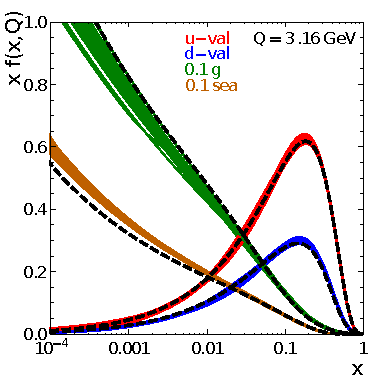
\includegraphics[width=0.5\textwidth]{CT10_1}}
   \subfloat[]{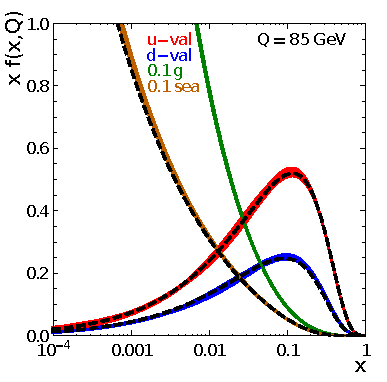
\includegraphics[width=0.5\textwidth]{CT10_2}}
   \caption[CT10 NNLO parton distribution functions]{CT10 NNLO parton distribution functions for up and down quarks,
   gluons and sea quarks, given at two factorisation scales: (a) Q = \SI{3.16}{\GeV}, (b) Q = \SI{85}{\GeV}
   \autocite{CT10_NNLO}.}
   \label{fig:CT10_PDFs}
\end{figure}

The total \ttbar production cross section for hard scattering processes in hadron collisions can be calculated to a
fixed order as \autocite{Sterman1986, primer_LHC}:
\begin{equation}
\sigma^{\ttbar} (s,\mtop^2) = \sum_{i,j} \int dx_i dx_j f_i(x_i, \mu_f^2) f_j(x_j,\mu_f^2) \hat{\sigma}_{i,j
\rightarrow \ttbar} (\hat{s}, \mtop^2, \alpha_S(\mu_r^2)),
\end{equation}
where the indices $i,j$ run over the incoming partons (gluons and quark-antiquark pairs), $x_{i,j}$ are the momentum
fractions of the incoming partons, $f_{i,j}$ are their parton distribution functions, and $\hat{\sigma}_{i,j
\rightarrow \ttbar}$ is the cross section of interacting partons, which depends on the parton centre of mass energy
$\hat{s} \sim x_i x_j s$, the top quark mass \mtop, and the QCD strong coupling constant $\alpha_S$. The latter
parameter is evaluated at renormalisation scale $\mu_r$. The top quark mass \mtop, as discussed in
Section~\ref{ss:top_mass}, also depends on the choice of renormalisation scheme and scale $\mu_r$.

The partonic cross section $\hat{\sigma}_{i,j\rightarrow \ttbar}$ can be calculated as a power series expansion in
$\alpha_S$ to different orders. If the calculation is performed in the lowest order of $\alpha_S$, it is referred to as
the leading order calculation (LO). Such calculations provide a very limited prediction power, since they do not include
any additional final-state partons produced in the hard scattering process. Moreover, LO calculations have a large
uncertainty from the renormalisation scale ambiguity. Inclusion of higher-order terms in the calculation decreases this
uncertainty, and a substantially better level of precision can be obtained with next-to-leading-order (NLO) and
next-to-next-to-leading-order (NNLO) calculations, which have recently become available for the \ttbar production
process.

The results of the most recent theoretical calculation of \ttbar cross section performed with NNLO QCD corrections
\autocite{NNLO_ttbar} are given in Table~\ref{tab:ttbar_NNLO_xsections}. The cross section has also been measured by CMS
and ATLAS experiments at the LHC -- the comparison of these measurements with the theoretical predictions at different
centre of mass energies is shown in Figure~\ref{fig:xsections_comparison_NNLO}.

\begin{table}[!hbp]
\centering
\caption{Theoretical predictions for \ttbar production cross section at
different LHC centre of mass energies, calculated at
next-to-next-to-leading-order (NNLO) \autocite{NNLO_ttbar}. The scales uncertainty corresponds to the choice of factorisation and renormalisation scales. }
\label{tab:ttbar_NNLO_xsections} 
\begin{tabular}{lrrr}
 \toprule
 $\sqrt{s}$ & $\sigma_\textrm{total}$ [\pb] & scales [\pb] & PDF [\pb] \\
 \midrule
 \SI{7}{\TeV}  & 172.0 & ${}^{+4.4~(2.6\%)}_{-5.8~(3.4\%)}$ & ${}^{+4.7~(2.7\%)}_{-4.8~(2.8\%)}$ \\
 \addlinespace[0.5em]
 \SI{8}{\TeV}  & 245.8 & ${}^{+6.2~(2.5\%)}_{-8.4~(3.4\%)}$ & ${}^{+6.2~(2.5\%)}_{-6.4~(2.6\%)}$ \\
 \addlinespace[0.5em]
 \SI{14}{\TeV} & 953.6 & ${}^{+22.7~(2.4\%)}_{-33.9~(3.6\%)}$ & ${}^{+16.2~(1.7\%)}_{-17.8~(1.9\%)}$ \\
 \bottomrule
\end{tabular}
\end{table}

\begin{figure}[bhtp]
   \centering
   {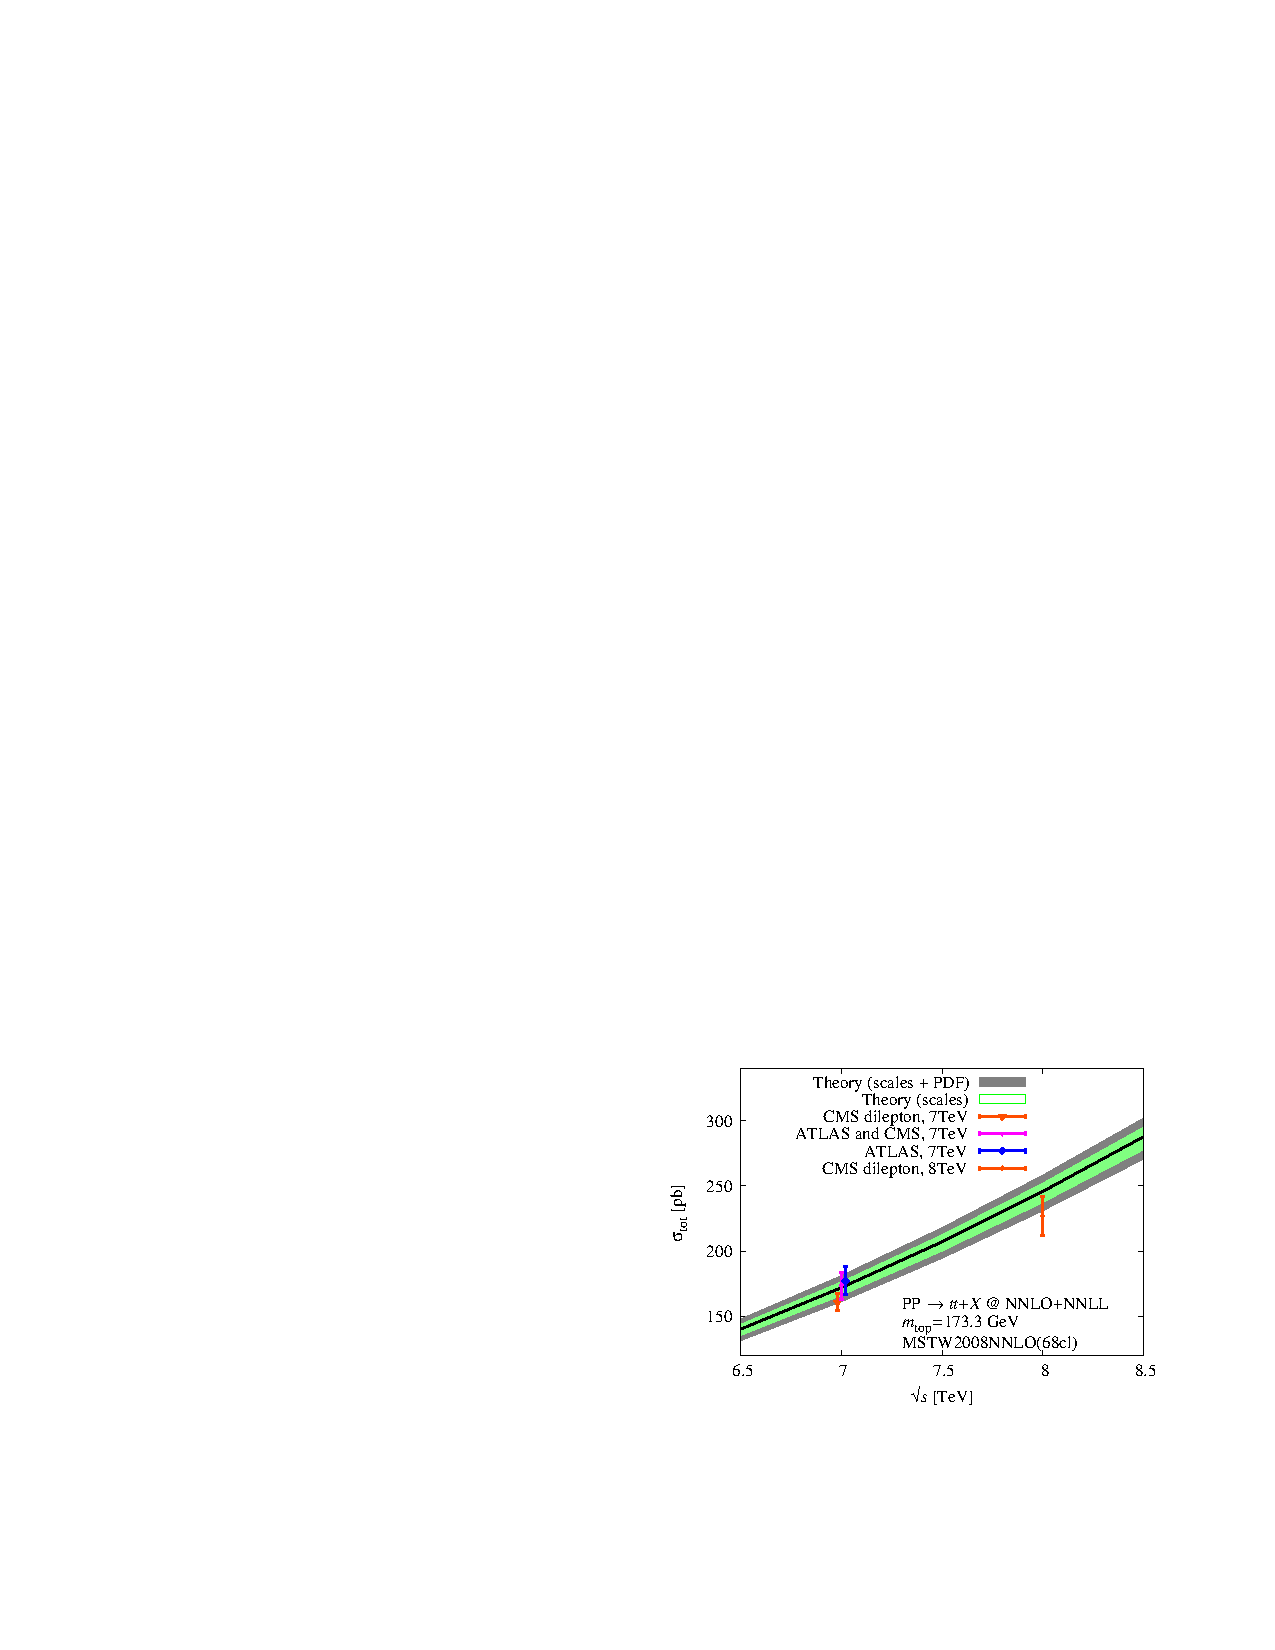
\includegraphics[width=0.65\textwidth]{xsections_comparison_NNLO}}
   \caption[Measurement of the \ttbar production cross section]{Measurement of the \ttbar production cross section at
   centre of mass energies of \SI{7}{\TeV} and \SI{8}{\TeV} by ATLAS and CMS experiments, compared with the theoretical
   predictions \autocite{NNLO_ttbar}.}
   \label{fig:xsections_comparison_NNLO}
\end{figure}

An abundance of top quark events at the LHC allows measurements of differential \ttbar production cross section with
respect to many different variables. These measurements provide important tools for validation of various MC models and
higher-order QCD calculations of \ttbar production. Since the very same models are used in BSM searches where \ttbar
events represent a major background, such validation is of great importance. Moreover, these measurements can themselves
be sensitive to signal contributions from new physics.

Normalised differential cross section in each bin $i$ of an observed variable $\mathrm{X}$ is given by:
\begin{equation}
\label{eq:normalised_differential_xsection_theory}
\frac{1}{\sigttbar^\mathrm{tot}} \frac{\mathrm{d}\sigma_i}{\mathrm{d} \mathrm{X}} = \frac{1}{\sigttbar^\mathrm{tot}}
\frac{x_i}{\Delta \mathrm{X}_i \calL},
\end{equation}
where $x_i$ is the number of signal events in data after subtraction of background, corrected for detector efficiency,
acceptance and migration between the bins of the variable $\mathrm{X}$; $\calL$ is the total integrated luminosity;
$\Delta \mathrm{X}_i$ is the variable bin width; and $\sigttbar^\mathrm{tot}$ is the total \ttbar production cross
section. The normalisation is performed in order to cancel the systematic uncertainties that are correlated between the
bins.

Both ATLAS and CMS collaborations have delivered a range of differential \ttbar production cross section measurements
\autocite{ATLAS_diff_xsections_7TeV, CMS_diff_xsections_7TeV}. For instance, Figure~\ref{fig:ATLAS_CMS_diff_xsections}
shows the normalised differential cross section with respect to the invariant mass of \ttbar pair ($m_{\ttbar}$),
measured by ATLAS and CMS collaborations using the $\sqrt{s} = \SI{7}{\TeV}$ LHC data. These measurements require a full
kinematic reconstruction of the semileptonic \ttbar decay in order to accurately calculate the $m_{\ttbar}$ variable.
Other variables requiring the kinematic reconstruction include the transverse momenta of top quarks decaying either
leptonically or hadronically, their rapidities, etc.

\begin{figure}[hbtp]
   \centering
   \subfloat[]{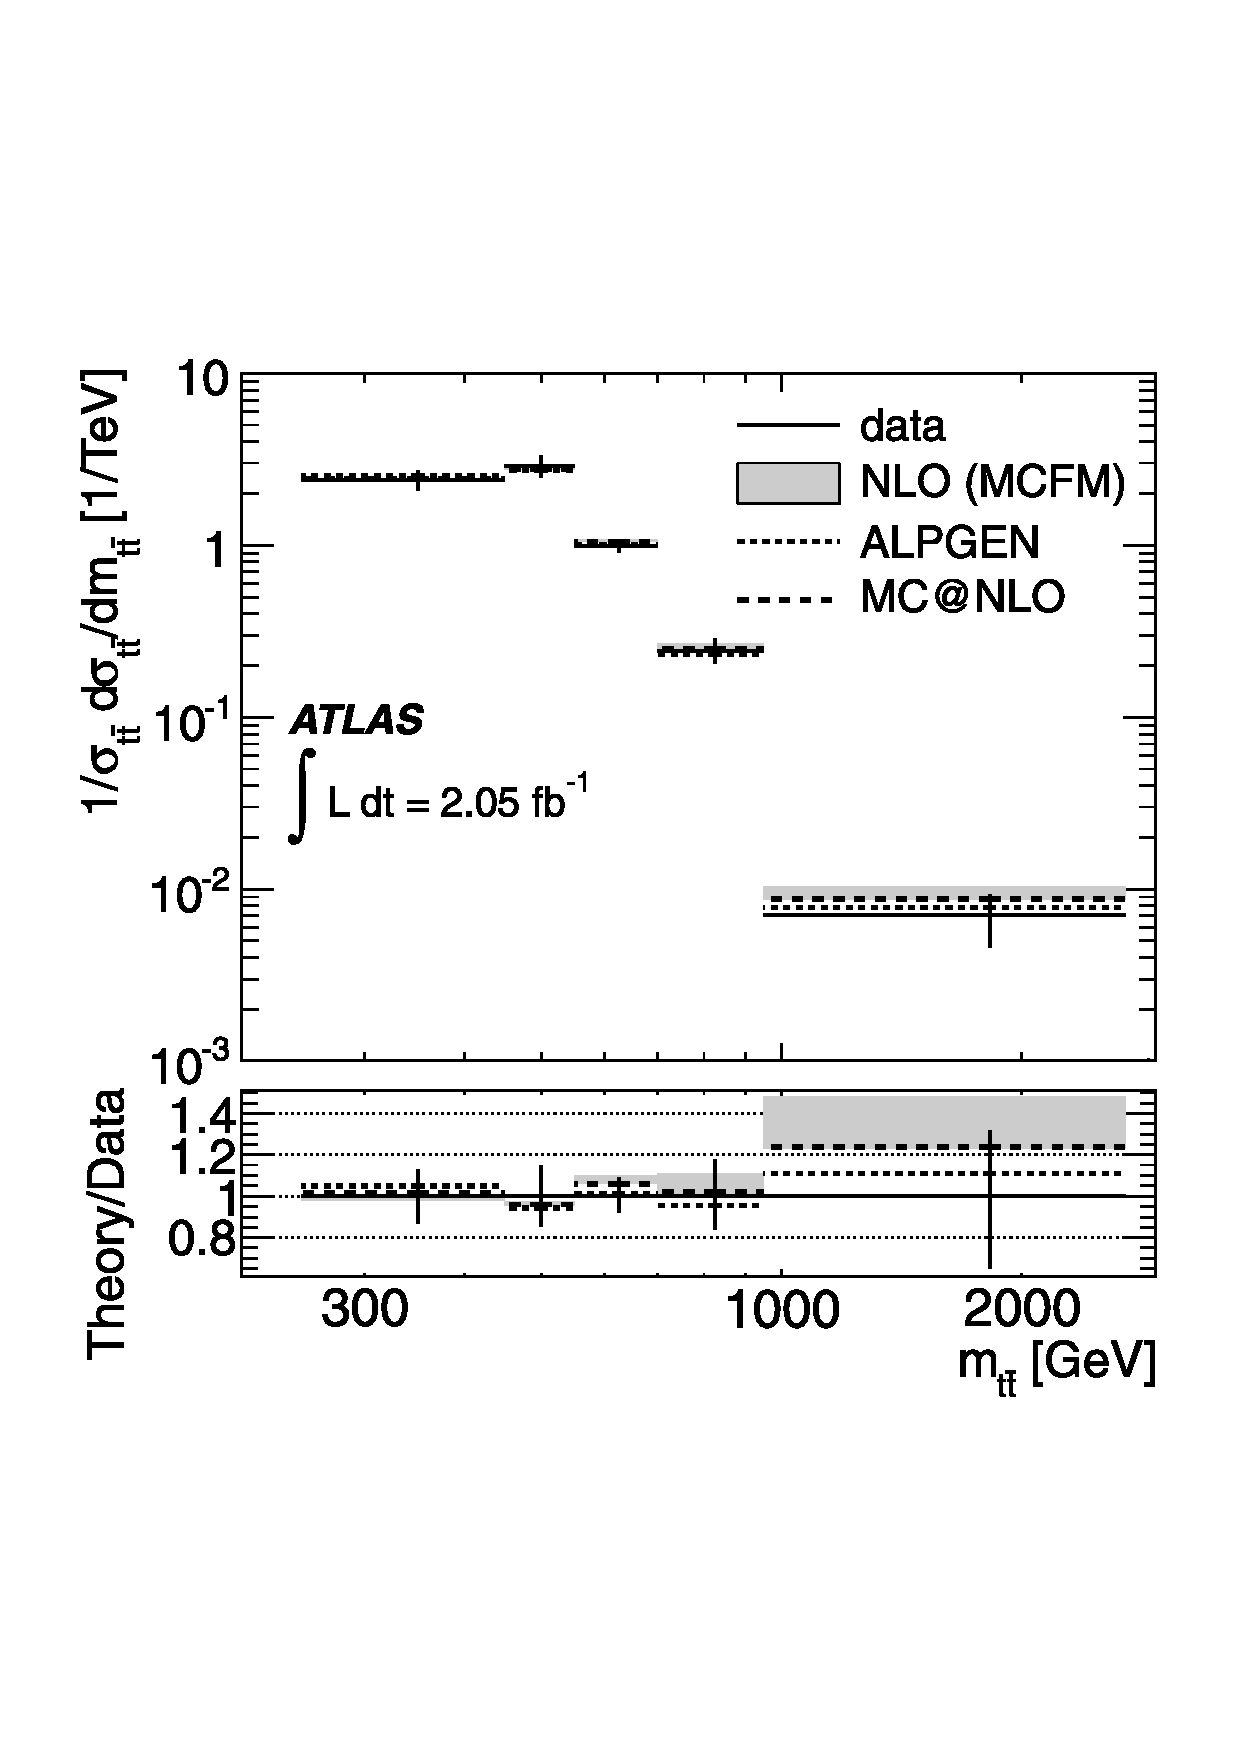
\includegraphics[width=0.5\textwidth]{ATLAS_diff_xsection_mtt}}
   \subfloat[]{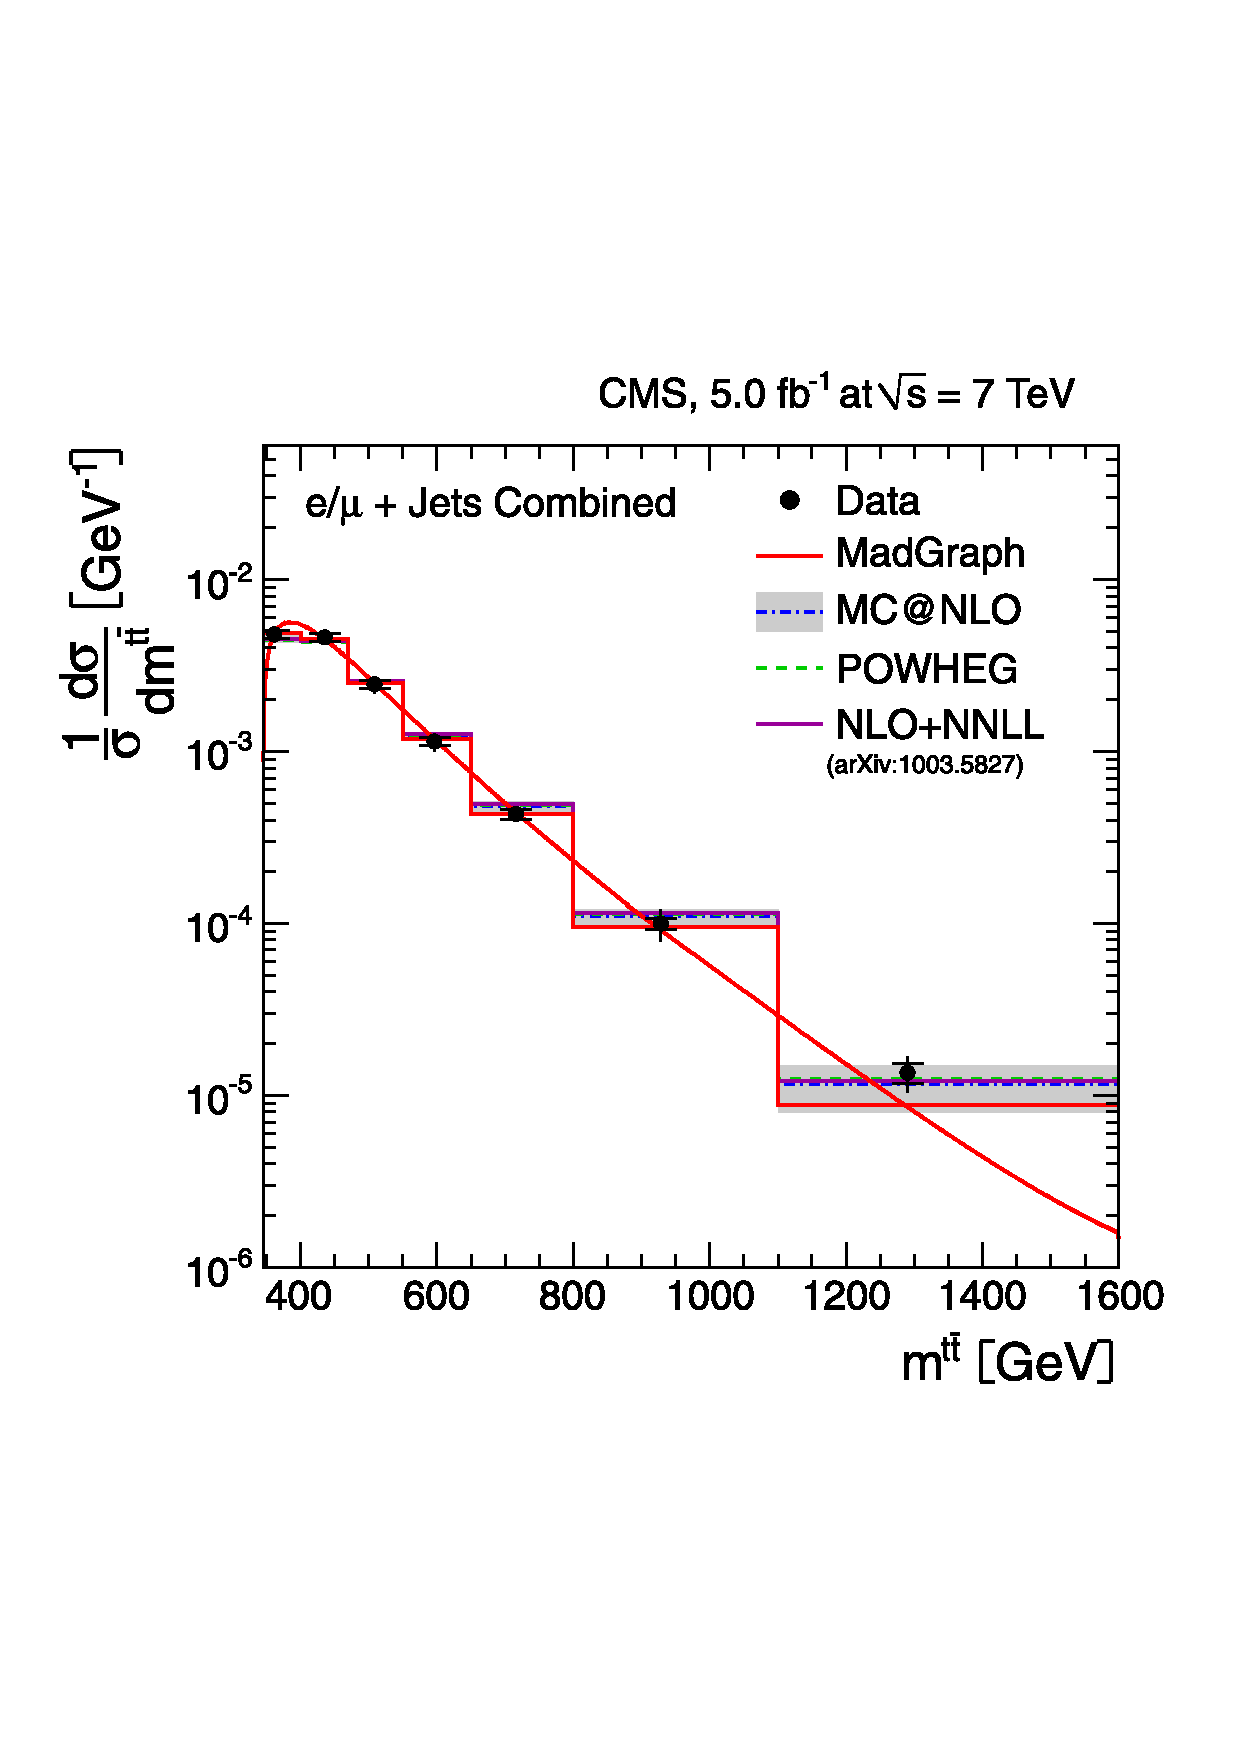
\includegraphics[width=0.5\textwidth]{CMS_diff_xsection_mtt}}
   \caption[Normalised differential \ttbar production cross section measurements by ATLAS and CMS
   collaborations]{Normalised differential \ttbar production cross section measurements in the $l+$jets channel with
   respect to the invariant mass of a top quark pair. (a) ATLAS measurement \autocite{ATLAS_diff_xsections_7TeV}, (b)
   CMS measurement \autocite{CMS_diff_xsections_7TeV}.}
   \label{fig:ATLAS_CMS_diff_xsections}
\end{figure}

In this thesis, the \ttbar differential cross section is measured with respect to so-called event-level (or global)
variables, not requiring a kinematic reconstruction of the \ttbar decay -- for example, missing transverse energy (\MET)
or total hadronic activity (\HT) in the event (see Section~\ref{ss_xsection:variables}). The main advantage of these
measurements is the absence of the systematic uncertainty associated with the kinematic reconstruction. Additionally,
signs of new physics scenarios could be revealed in the tails of these distributions. For example, an associated
production of a \ttbar pair with some new resonance ($\ttbar+\mathrm{X}$) decaying invisibly can show up in the tail of
the missing transverse energy distribution.

\section{Summary}
In this chapter, an overview of the Standard Model has been presented. The concept of the gauge principle and its
applications in the electroweak theory and the Quantum Chromodynamics, as well as the mechanism of the electroweak
symmetry breaking have been briefly described. Shortcomings of the Standard Model and some models proposing the
solutions have been mentioned. Finally, an introduction to top quark physics has been given, pointing out the relevance
and importance of the top quark mass and differential cross section measurements presented in this thesis.

%%% Local Variables: 
%%% mode: latex
%%% TeX-master: "../thesis"
%%% End: 
